\documentclass[12pt, letterpaper]{article}
\usepackage[utf8]{inputenc}
\usepackage{graphicx}
\usepackage{xcolor}
\usepackage{hyperref}
\definecolor{darkblue}{rgb}{0.0, 0.0, 0.55}
\hypersetup{
    colorlinks=true,
    linkcolor=darkblue,
    filecolor=darkblue,
    urlcolor=darkblue,
    citecolor=darkblue
}
\usepackage{amsmath}
\usepackage{booktabs}
\usepackage{caption}
\usepackage{geometry}
\usepackage{natbib}
\usepackage{tabularx}
\geometry{margin=1in}

\title{Stay, React, or Conform? Examining Social Influence Effects on Aesthetic Judgments}
\author{Omar Lizardo \& Sara Skiles}
\date{Revised Manuscript --- \today}

\begin{document}

\maketitle

\begin{abstract}
In this study, we address the question, foundational to sociological studies of taste, of the extent to which others' aesthetic judgments causally influence individual evaluations of cultural works, and how this influence depends on the social distance between self and other. While past research has documented observational associations between cultural tastes and social networks, the underlying causal mechanisms—whether individuals actively conform, react, or remain anchored in their initial judgments—have rarely been submitted to experimental test. Using a national survey experiment ($N = 2,275$), we manipulate exposure to others' aesthetic evaluations (likes vs.\ dislikes) and the status characteristics of the evaluating group across repeated trials. Using a difference-in-differences framework and inverse probability weighting, we find substantial evidence of \textit{valence asymmetry}: while negative evaluations from others broadly suppress positive exposure drift across groups, positive evaluations facilitate upward shifts conditionally based on status congruence. Furthermore, analyzing discrete behavioral choices shows that evaluative stability (``staying'') is not driven by high status alone, but by \textit{structural status consistency}: both high-consistent and low-consistent individuals display high evaluative inertia, whereas status-inconsistent individuals exhibit evaluative fluidity.
\end{abstract}

\newpage
\section{Introduction}

\subsection{Theoretical Background}
Taste expressions and consumption have long been shown to be a function of individuals' desire to differentiate themselves from others \citep{simmel1957, dimaggio1987}. \citet{bourdieu1984} suggests that taste differences evoke a visceral reaction, and it is through the rejection of others' aesthetic tastes that individuals engage in the symbolic boundary work that separates them. Thus, the expression of distastes serves to communicate social distance from certain social groups \citep{bryson1996, lamont2002}. In contexts where individuals discover a similarity in taste with members of a meaningful outgroup, they frequently engage in ``taste abandonment'' to maintain social boundaries \citep{berger2008}, while contexts in which individuals find a similarity of tastes with members of their ingroup can foster community and solidarity \citep{wohl2015community-2d2, vanzella2022tastes}.

Despite the rich sociological literature linking cultural tastes and network ties \citep{erickson1996, lizardo2006}, this body of work has almost exclusively relied on static, cross-sectional, and observational survey data. Consequently, observational homophily inevitably conflates prior social sorting, shared environmental exposure, and active social influence. This leaves open a fundamental causal question: \textit{How does direct access to the evaluations of others causally alter our own aesthetic judgments in real time?}

To answer this question, we build a theoretical framework that integrates three distinct mechanisms. First, in situations of aesthetic ambiguity, others' choices provide heuristic information to resolve uncertainty \citep{strang2001search-10a, salganik2006experimental-88d}. However, we expect a pronounced \textit{valence asymmetry}: negative evaluations from others act as a potent suppressive veto that halts the positive exposure drift observed under repeated evaluation, whereas positive evaluations act selectively depending on social status alignment.

Second, cultural influence is conditioned by the status of the evaluator relative to the self \citep{heider1946attitudes-ff3, bourdieu1984, lizardo2016cultural-aaa}. We examine whether individuals show same-status alignment, upward conformity to high-status cultural specialists, or reactive distancing from low-status evaluations.

Third, beyond linear mean shifts, individuals differ in their inertial propensity to maintain their initial judgment (``staying''). Drawing on status crystallization theory \citep{lenski1954status}, we propose that structural consistency between objective educational capital and subjective class identification produces cognitive certainty and evaluative inertia, whereas status inconsistency induces evaluative fluidity.

\subsection{Hypotheses}
\subsubsection{Mere Exposure and Positive Drift}
For participants in the Control Condition who are simply asked to rate the painting twice without being exposed to the opinions of others, repeated exposure to a cultural object across trials is expected to produce an upward drift in evaluation even in the absence of external social information, a phenomenon in psychology known as the \textit{mere exposure effect} \citep{zajonc1968attitudinal, reber1998effects-efe}.\footnote{For an application of the mere exposure effect to historical dynamics in the aesthetic evaluation of art see \citet{cutting2003gustave}.} So our baseline hypothesis is simply that we should observe such positive drift, with participants who are asked to judge the same cultural object twice being more likely to produce a more positive judgment (on average) the second time around. 

\subsubsection{Social Influence and Generalized Alignment}

External social cues then either facilitate or suppress this exposure drift. In the case of generalized influence without status cues, exposure to positive evaluations from others is expected to enhance this positive exposure drift, whereas exposure to negative evaluations from others is expected to suppress it \citep{salganik2006experimental-88d}. Accordingly, we should expect (\textit{Hypothesis 1}) that individuals will \textit{adjust} their judgments to align with the aggregate evaluations of others, shifting positively when provided information that others like the object and negatively when provided information that others dislike it. 

\subsubsection{Cultural Goodwill and Asymmetric Alignment}
Following Bourdieu's \citeyearpar{bourdieu1984} idea of ``cultural goodwill,'' we should expect (\textit{Hypothesis 2}) lower-status respondents to be more likely to \textit{align} their judgments with those of high-status others, such that they will tend to move towards more positive evaluations when provided information that high-status others liked the cultural object, and towards negative evaluations when provided information that high-status others disliked the painting. 

\subsubsection {Status-Based Distancing and Asymmetric Disalignment}

An alternative hypothesis, based on the idea of \textit{reactance} and distancing from the judgments of others of different status, particularly when it comes to high-status individuals distancing themselves from the judgments of low-status others \citep{bourdieu1984}. Accordingly, we should expect (\textit{hypothesis 3}) that high-status individuals will shift away from the judgments of low-status individuals, moving towards dislike when provided with information that low-status others liked the cultural object, and towards liking when provided with information that low-status others disliked the painting. 

\subsubsection{Status Inconsistency and Aesthetic Malleability}

Finally, with regard to status crystallization and status inconsistency \citep{hope1975models}, we should expect (\textit{Hypothesis 4}) individuals with consistent status profiles (e.g., Middle Class with College or Working Class without College) to exhibit a higher propensity to maintain their initial evaluation (``staying'') than status-inconsistent individuals, whose judgments should be more malleable given information on the aesthetic opinions of others.  

\section{Data and Methods}

\subsection{Sample Recruitment and Survey Administration}
Data for this study were collected between February 28 and March 6, 2012, via an online experimental survey administered by Survey Sampling International (SSI), a leading research firm specializing in online panel recruitment and survey sampling. A total of 3,782 panel members accessed the survey instrument. Of these, 97 were excluded due to lack of informed consent ($N = 85$) or age under 18 ($N = 12$), 1,394 were screened out because demographic quota targets had already been met, and 16 dropped out during early screens, resulting in an analytic sample of $N = 2,275$ completed responses (with $N = 2,253$ providing complete initial and post-treatment evaluations). Participants received monetary compensation (\$3.92) via SSI, funded by an NSF Doctoral Dissertation Improvement Grant (Award SES-1203426) and the University of Notre Dame Institute for Scholarship in Liberal Arts.

The sampling frame employed dynamic quota matching calibrated against U.S. Census benchmarks for gender, age, race/ethnicity, and geographic region to achieve a diverse and quasi-representative national sample of U.S. adults. To ensure adequate statistical power for examining status-differentiated cultural dynamics—particularly within high-cultural-capital occupational cells, the sample incorporated a deliberate oversample of college graduates (40.5\% holding a bachelor's degree or higher in the sample versus approximately 28\% nationally in 2012). Table \ref{tbl:descriptives} presents the full demographic breakdown of the sample, compared with U.S. population parameters, separated by experimental treatment condition.

\subsection{Inferential Scope and Interpretation of Confidence Intervals}
Because the survey used a quota-matched, opt-in online consumer panel rather than a strict probability-based sample with known inclusion probabilities (such as the GSS or ANES), the reported standard errors, $p$-values, and confidence intervals should be interpreted as reflecting \textit{model-based and experimental design uncertainty within the sample}, rather than formal design-based population parameter estimates. 

The randomization mechanism built into the Qualtrics survey engine ensures that internal validity is maximized: respondents were randomly assigned to treatment and control conditions, creating balanced experimental groups across all observed baseline characteristics (Table \ref{tbl:descriptives}). At the same time, the demographic diversity across gender, age, race, and geographic region provides substantial ecological validity and heterogeneity compared to conventional undergraduate convenience samples. 

Because cell sample sizes vary across experimental conditions and observational status consistency subgroups, we also report a comprehensive Minimum Detectable Effect (MDE) power analysis in Appendix \ref{sec:appendix_power_mde} (Table \ref{tbl:mde_analysis} and Figure \ref{fig:mde_curves}), explicitly delineating the statistical precision and empirical detection boundaries of the experimental design.

\begin{table}[ht!]
\centering
\small
\caption{Demographic Characteristics of Survey Sample Compared to U.S. Population Benchmarks}
\label{tbl:descriptives}
\setlength{\tabcolsep}{4.5pt}
\begin{tabular*}{\linewidth}{@{\extracolsep{\fill}}lcccccc@{}}
\toprule
Demographic Variable & Sample $N$ & Sample \% & U.S. Pop \% & Treatment & No Alter & Taste Only \\
\midrule
\textbf{Gender} & & & & & & \\
\quad Women & 1,184 & 52.1\% & 51.5\% & 51.7\% & 52.2\% & 53.9\% \\
\quad Men & 1,091 & 47.9\% & 48.5\% & 48.3\% & 47.8\% & 46.1\% \\
\addlinespace[3pt]
\textbf{Race / Ethnicity} & & & & & & \\
\quad White & 1,463 & 64.3\% & 65.1\% & 64.7\% & 63.2\% & 63.1\% \\
\quad Hispanic / Latino & 365 & 16.1\% & 15.8\% & 16.2\% & 14.8\% & 15.9\% \\
\quad Black / African American & 279 & 12.3\% & 12.3\% & 12.1\% & 13.7\% & 12.1\% \\
\quad Asian / Pacific Islander & 103 & 4.5\% & 4.5\% & 4.4\% & 5.5\% & 4.6\% \\
\quad Other / Multiracial & 65 & 2.8\% & 2.3\% & 2.5\% & 2.7\% & 4.3\% \\
\addlinespace[3pt]
\textbf{Age Group} & & & & & & \\
\quad 18--24 & 272 & 12.0\% & 13.1\% & 11.9\% & 11.0\% & 12.7\% \\
\quad 25--34 & 410 & 18.0\% & 17.5\% & 18.2\% & 16.5\% & 17.9\% \\
\quad 35--44 & 402 & 17.7\% & 17.5\% & 17.9\% & 13.7\% & 18.7\% \\
\quad 45--54 & 441 & 19.4\% & 19.2\% & 19.4\% & 20.9\% & 18.4\% \\
\quad 55--64 & 372 & 16.3\% & 15.6\% & 16.5\% & 15.4\% & 16.1\% \\
\quad 65+ & 377 & 16.6\% & 17.2\% & 16.1\% & 22.5\% & 16.2\% \\
\addlinespace[3pt]
\textbf{Geographic Region} & & & & & & \\
\quad Northeast & 417 & 18.3\% & 17.9\% & 18.8\% & 16.5\% & 17.0\% \\
\quad South & 816 & 35.9\% & 37.2\% & 36.6\% & 39.6\% & 30.5\% \\
\quad Midwest & 505 & 22.2\% & 21.6\% & 21.2\% & 26.4\% & 24.8\% \\
\quad West & 536 & 23.6\% & 23.3\% & 23.4\% & 17.6\% & 27.7\% \\
\addlinespace[3pt]
\textbf{Education (Oversampled)} & & & & & & \\
\quad Less than High School & 89 & 3.9\% & 13.3\% & 3.8\% & 3.3\% & 4.6\% \\
\quad High School Diploma & 474 & 20.8\% & 30.4\% & 20.3\% & 23.6\% & 21.9\% \\
\quad Some College / AA & 791 & 34.8\% & 28.5\% & 36.0\% & 31.3\% & 30.6\% \\
\quad Bachelor's Degree & 625 & 27.5\% & 18.1\% & 27.3\% & 27.5\% & 28.5\% \\
\quad Graduate / Professional & 296 & 13.0\% & 9.6\% & 12.6\% & 14.3\% & 14.5\% \\
\midrule
\textbf{Total $N$} & \textbf{2,275} & \textbf{100.0\%} & & \textbf{1,746} & \textbf{182} & \textbf{347} \\
\bottomrule
\end{tabular*}
\begin{minipage}{\linewidth}
\vspace{4pt}
\footnotesize
\textit{Note:} U.S. population benchmarks are drawn from the 2010/2012 U.S. Census Bureau Current Population Survey (CPS). The analytic sample oversamples college-educated respondents to populate higher-status occupational cells.
\end{minipage}
\end{table}

\subsection{Experimental Design and Stimulus}
All respondents viewed an image of the same artwork: \textit{Nocturne: Blue and Gold -- Old Battersea Bridge} by James McNeill Whistler (1872), displayed in Figure \ref{fig:stimulus}. The painting was selected based on an online pilot study ($N=100$) testing eight artworks; the Whistler painting was chosen because it generated the highest initial pre-treatment variance in aesthetic evaluations across all demographic subgroups.

\begin{figure}[ht!]
    \centering
    
\includegraphics[width=0.55\textwidth]{figures/experimental_stimulus.jpeg}
    \caption{Experimental Stimulus: \textit{Nocturne: Blue and Gold -- Old Battersea Bridge}, by James McNeill Whistler (1872)}
    \label{fig:stimulus}
\end{figure}

The experiment used an incomplete factorial design with within-subject pre/post trials. In Trial 1, respondents provided their pre-treatment baseline rating of the painting on a 7-point Likert scale (1 = ``Dislike it very much'', 4 = ``Neither like nor dislike'', 7 = ``Like it very much''). Next, during an intervening survey block, respondents completed demographic questions and a musical taste battery before treatment respondents read a brief vignette describing how a group of other people evaluated the artwork. Finally, in Trial 2, respondents were shown the painting again and provided their second evaluation.

To prevent terminological confusion, we distinguish between the \textit{pre-treatment baseline measurement} (Trial 1, which captures initial, uninfluenced aesthetic preference) and the \textit{Control Condition} (the experimental group that receives no information about others between trials, allowing us to observe pure temporal re-evaluation in the absence of treatment). We refer to changes over repeated trials in this unexposed group as \textit{exposure drift}.

\subsection{Mitigation of Experimenter Demand Characteristics and Respondent Reactivity}
A common methodological concern in within-subject experimental designs is whether respondents become aware that an evaluative shift is being measured, inducing experimenter demand compliance or artificial consistency. We implemented four procedural and design safeguards to mitigate demand awareness and assess respondent reactivity.

First, Trial 1 and Trial 2 were separated by an extensive cognitive and temporal buffer comprising 15 to 20 minutes of substantive survey batteries. Between aesthetic evaluations, respondents completed detailed modules on educational history, parental degree attainment, employment status, 22-category Standard Occupational Classification (SOC) coding, annual household income, and a comprehensive 20-genre musical taste battery evaluating preference ratings, listening frequency, and listener demographic stereotypes. This substantial intervening distance prevented respondents from mechanically recalling or feeling compelled to repeat their Trial 1 ratings.

Second, the experimental feedback screens were framed naturalistically as observational descriptive summaries from prior survey waves rather than prescriptive social norms: respondents were told, \textit{``Our survey so far indicates that the group of people most likely to say that they [LIKE / DISLIKE] the painting you saw have completed\dots''} Immediately following this prompt, respondents completed attribution and subjective similarity probes concerning the evaluating group, maintaining the perception that the survey was investigating social perception rather than testing their personal susceptibility to persuasion. At no point were participants prompted to re-evaluate their prior rating or instructed that conformity was expected.

Third, in the following analyses, all treatment shifts are compared against the unexposed Control Condition. Because control respondents completed the identical intervening survey battery without receiving any cue from others, comparing treatment conditions against this baseline cleanly separates genuine informational influence from any residual re-test reactivity or temporal fatigue.

Finally, the empirical distribution of discrete behavioral choices provides powerful evidence against demand compliance. Over 74\% of respondents across conditions exhibited complete evaluative stability (``staying''), and a substantial proportion displayed active oppositional reactance by shifting in the direction opposite to the cue. Had respondents been compliance-driven, conformity rates would have dominated across conditions rather than emerging selectively within specific status-inconsistent configurations.

\subsection{Variables and Measurement}
Aesthetic evaluation was measured on a reversed 1--7 scale. In continuous models, the outcome is the repeated evaluation across trials. In behavioral models, change between trials is categorized into three mutually exclusive choices: \textit{Stay} ($\Delta = 0$), \textit{Conform} (moving in the direction of others' evaluations), and \textit{React} (moving in the opposite direction).

The treatment conditions crossed others' evaluation (Like vs.\ Dislike) with others' social status. High-status others were differentiated into Cultural Specialists (possessing multiple advanced degrees including a PhD and working in higher education) and Economic Specialists (holding a bachelor's degree in business and working in financial investment). Low-status others were described as possessing a high school education and working in food service. In addition, two Taste-Only conditions provided others' like or dislike evaluations without any status indicators, and a pure Control Condition provided no information about others between trials ($N=182$).

To capture respondents' structural social location, we examine objective educational attainment (College Degree vs.\ No College) and subjective class self-identification (Middle Class vs.\ Working Class). Methodologically, we analyze these dimensions stepwise: we first evaluate the separate moderating effects of educational attainment alone and subjective class identification alone (Section \ref{sec:stepwise_models}, Figure \ref{fig:did_edu_class}, and Table \ref{tbl:did_edu_class}) before examining their intersection in a four-quadrant typology of status consistency: Working Class without College, Working Class with College, Middle Class without College, and Middle Class with College. Furthermore, to verify that our substantive conclusions are not sensitive to the boundary demarcations of subjective class, we evaluate an alternative categorization restricting the sample strictly to self-identified working- and middle-class respondents (excluding lower- and upper-class extremes) as an additional sensitivity analysis in Appendix \ref{sec:appendix_class_robustness}.

A key methodological challenge in experimental designs that examine status-contingent influence arises from the hybrid nature of the design. While the experimental cues (others' evaluation valence and others' status) were randomly assigned, respondents' own social locations—captured by the crossing of educational attainment and subjective class identification—represent pre-existing, observational attributes \citep{cruces2013biases}. Consequently, individuals do not have an equal probability of belonging to each status group: for example, Middle Class individuals with a college degree are systematically older, more likely to have college-educated parents, and differ in racial/ethnic composition compared to non-college Working Class individuals. If unaddressed, comparisons across status groups (and their interactions with the randomized treatments) risk confounding the effect of social class with these correlated background characteristics.

To solve this problem and strengthen causal inference, we implement Inverse Probability Weighting (IPW) using generalized propensity scores \citep{rosenbaum1983central}. The logic of IPW proceeds in two steps. First, for each respondent, we estimate a multinomial logistic regression modeling the probability of belonging to their observed status consistency group $S_i \in \{1, 2, 3, 4\}$ conditional on exogenous baseline covariates $\mathbf{X}_i$ (age, gender, race/ethnicity, and parental educational capital): $e_s(\mathbf{X}_i) = P(S_i = s \mid \mathbf{X}_i)$. Second, each observation is weighted by the inverse of its estimated propensity score to target the Average Treatment Effect (ATE) across the pooled sample: $w_i = 1 / e_s(\mathbf{X}_i) = 1 / P(S_i = s \mid \mathbf{X}_i)$.

Intuitively, IPW creates a synthetic ``pseudo-population'' by up-weighting underrepresented demographic profiles within each status group (e.g., working-class respondents whose parents completed college) and down-weighting overrepresented profiles. This weighting scheme breaks the empirical association between the baseline covariates $\mathbf{X}_i$ and status group membership. Under the assumption of conditional exchangeability (no unmeasured confounders given $\mathbf{X}_i$) and positivity, IPW ensures that status groups are demographically comparable. As a result, subsequent differences in evaluative shifts, behavioral inertia, or reactance across status categories can be interpreted as the direct consequence of structural status location and status consistency, rather than demographic artifacts.

\subsection{Difference-in-Differences Analytic Strategy}
To strictly isolate information-induced shifts from repeated-measurement exposure drift, we formulate our analysis within a Difference-in-Differences (DiD) framework. Rather than examining simple pre-to-post changes within each condition in isolation—which conflates the effect of information from others with the natural exposure drift that occurs upon viewing an artwork a second time—the DiD strategy compares every treatment condition against the influence-unexposed Control Condition.

Accordingly, we specify a linear mixed-effects model with random intercepts for respondents of the form:
\begin{equation}
\begin{split}
\text{Taste}_{it} = {} & \beta_0 + \beta_{1} \text{Trial}_{it} + \sum_{k=2}^{K} \beta_{k} \text{Cond}_{ik} + \sum_{k=2}^{K} \delta_{k} (\text{Trial}_{it} \times \text{Cond}_{ik}) + u_i + \epsilon_{it}
\end{split}
\label{eq:did_model}
\end{equation}
where $i$ indexes individual respondents ($i = 1, \dots, N$), $t \in \{1, 2\}$ indexes measurement trials (Trial 1 pre-treatment baseline vs.\ Trial 2 post-treatment evaluation), $k \in \{1, \dots, K\}$ indexes the experimental conditions with the unexposed Control Condition ($k = 1$) serving as the omitted reference category, $u_i \sim \mathcal{N}(0, \sigma^2_u)$ is the individual-specific random intercept, and $\epsilon_{it} \sim \mathcal{N}(0, \sigma^2_\epsilon)$ is the trial-level residual error.

The intercept ($\beta_0$) represents the expected baseline aesthetic evaluation at Trial 1 (pre-treatment) for respondents assigned to the unexposed Control Condition: $\beta_0 = E[\text{Taste} \mid \text{Trial} = 1, \text{Control}]$. The Trial main effect ($\beta_{1}$) captures the counterfactual \textit{exposure drift} from Trial 1 to Trial 2 in the absence of external information from others: $\beta_{1} = E[\text{Taste} \mid \text{Trial} = 2, \text{Control}] - E[\text{Taste} \mid \text{Trial} = 1, \text{Control}]$. When repeated viewing induces an intrinsic appreciation of the artwork (the mere exposure effect), $\beta_{1}$ should be positive and statistically significant.

The condition main effects ($\beta_k$) reflect pre-treatment differences between condition $k$ and the Control Condition at Trial 1: $\beta_k = E[\text{Taste} \mid \text{Trial} = 1, \text{Cond} = k] - E[\text{Taste} \mid \text{Trial} = 1, \text{Control}]$. Because respondents were randomly assigned to experimental conditions before viewing the painting, these coefficients assess baseline balance and are expected to be close to zero. The interaction coefficients ($\delta_k$) represent the \textit{causal Difference-in-Differences treatment effects}. Each $\delta_k$ measures whether the change in evaluations from Trial 1 to Trial 2 in treatment condition $k$ differed significantly from the change observed in the unexposed Control Condition:
\begin{equation}
\begin{split}
\delta_k = {} & \left( E[\text{Taste} \mid \text{Trial} = 2, k] - E[\text{Taste} \mid \text{Trial} = 1, k] \right) \\
              & - \left( E[\text{Taste} \mid \text{Trial} = 2, \text{Control}] - E[\text{Taste} \mid \text{Trial} = 1, \text{Control}] \right)
\end{split}
\end{equation}

Substantively, $\delta_k$ answers the counterfactual question: \textit{Did exposure to evaluation $k$ cause respondents' aesthetic judgments to change significantly more or less than they would have changed under mere repeated exposure alone?} A positive estimate ($\delta_k > 0$) indicates that feedback from others facilitated aesthetic appreciation beyond natural exposure drift, whereas a negative estimate ($\delta_k < 0$) indicates that feedback from others suppressed or reversed the positive exposure drift that would have naturally occurred.\footnote{By the Frisch-Waugh-Lovell theorem, estimating Equation \ref{eq:did_model} via linear mixed models with individual random intercepts ($u_i$) is mathematically equivalent to regressing individual change scores ($\Delta \text{Taste}_i = \text{Taste}_{i2} - \text{Taste}_{i1}$) on the treatment indicators with the Control Condition as the omitted reference group:
\begin{equation}
\Delta \text{Taste}_i = \beta_{1} + \sum_{k=2}^{K} \delta_k \text{Cond}_{ik} + \epsilon_i
\end{equation}
where the intercept directly estimates the control exposure drift ($\beta_{1}$) and the condition slopes estimate the DiD treatment effects ($\delta_k$).} To examine non-linear behavioral choices, we also estimate multinomial logistic regressions modeling the discrete probabilities of Staying, Conforming, and Reacting.

\section{Results}

\subsection{Covariate Balance Across Observational Status Categories}
Before evaluating our focal hypotheses, we assessed the demographic comparability of the four observational status consistency groups. It is important to emphasize that while the experimental conditions (liking vs.\ disliking and status cues of others) were randomized and thus inherently balanced by design, respondents' own structural locations (Education and Subjective Social Class) are observational. 

Figure \ref{fig:balance} displays the standardized mean differences (SMD) for all baseline covariates across the status categories before and after Inverse Probability Weighting (IPW), generated using \texttt{cobalt} \citep{greifer2022cobalt}. Prior to weighting, status groups exhibited substantial demographic disparities: for instance, college-educated middle-class respondents had older ages and higher rates of parental college attainment (raw SMDs exceeding 0.35 to 0.50). Following IPW estimation, the weighted pseudo-population achieved balance, with all absolute standardized mean differences compressed well below the conventional conservative threshold of 0.10 standard deviations. This confirms that subsequent model estimates isolate the effect of social class and status consistency, net of observed demographic sorting.

\begin{figure}[ht!]
    \centering
    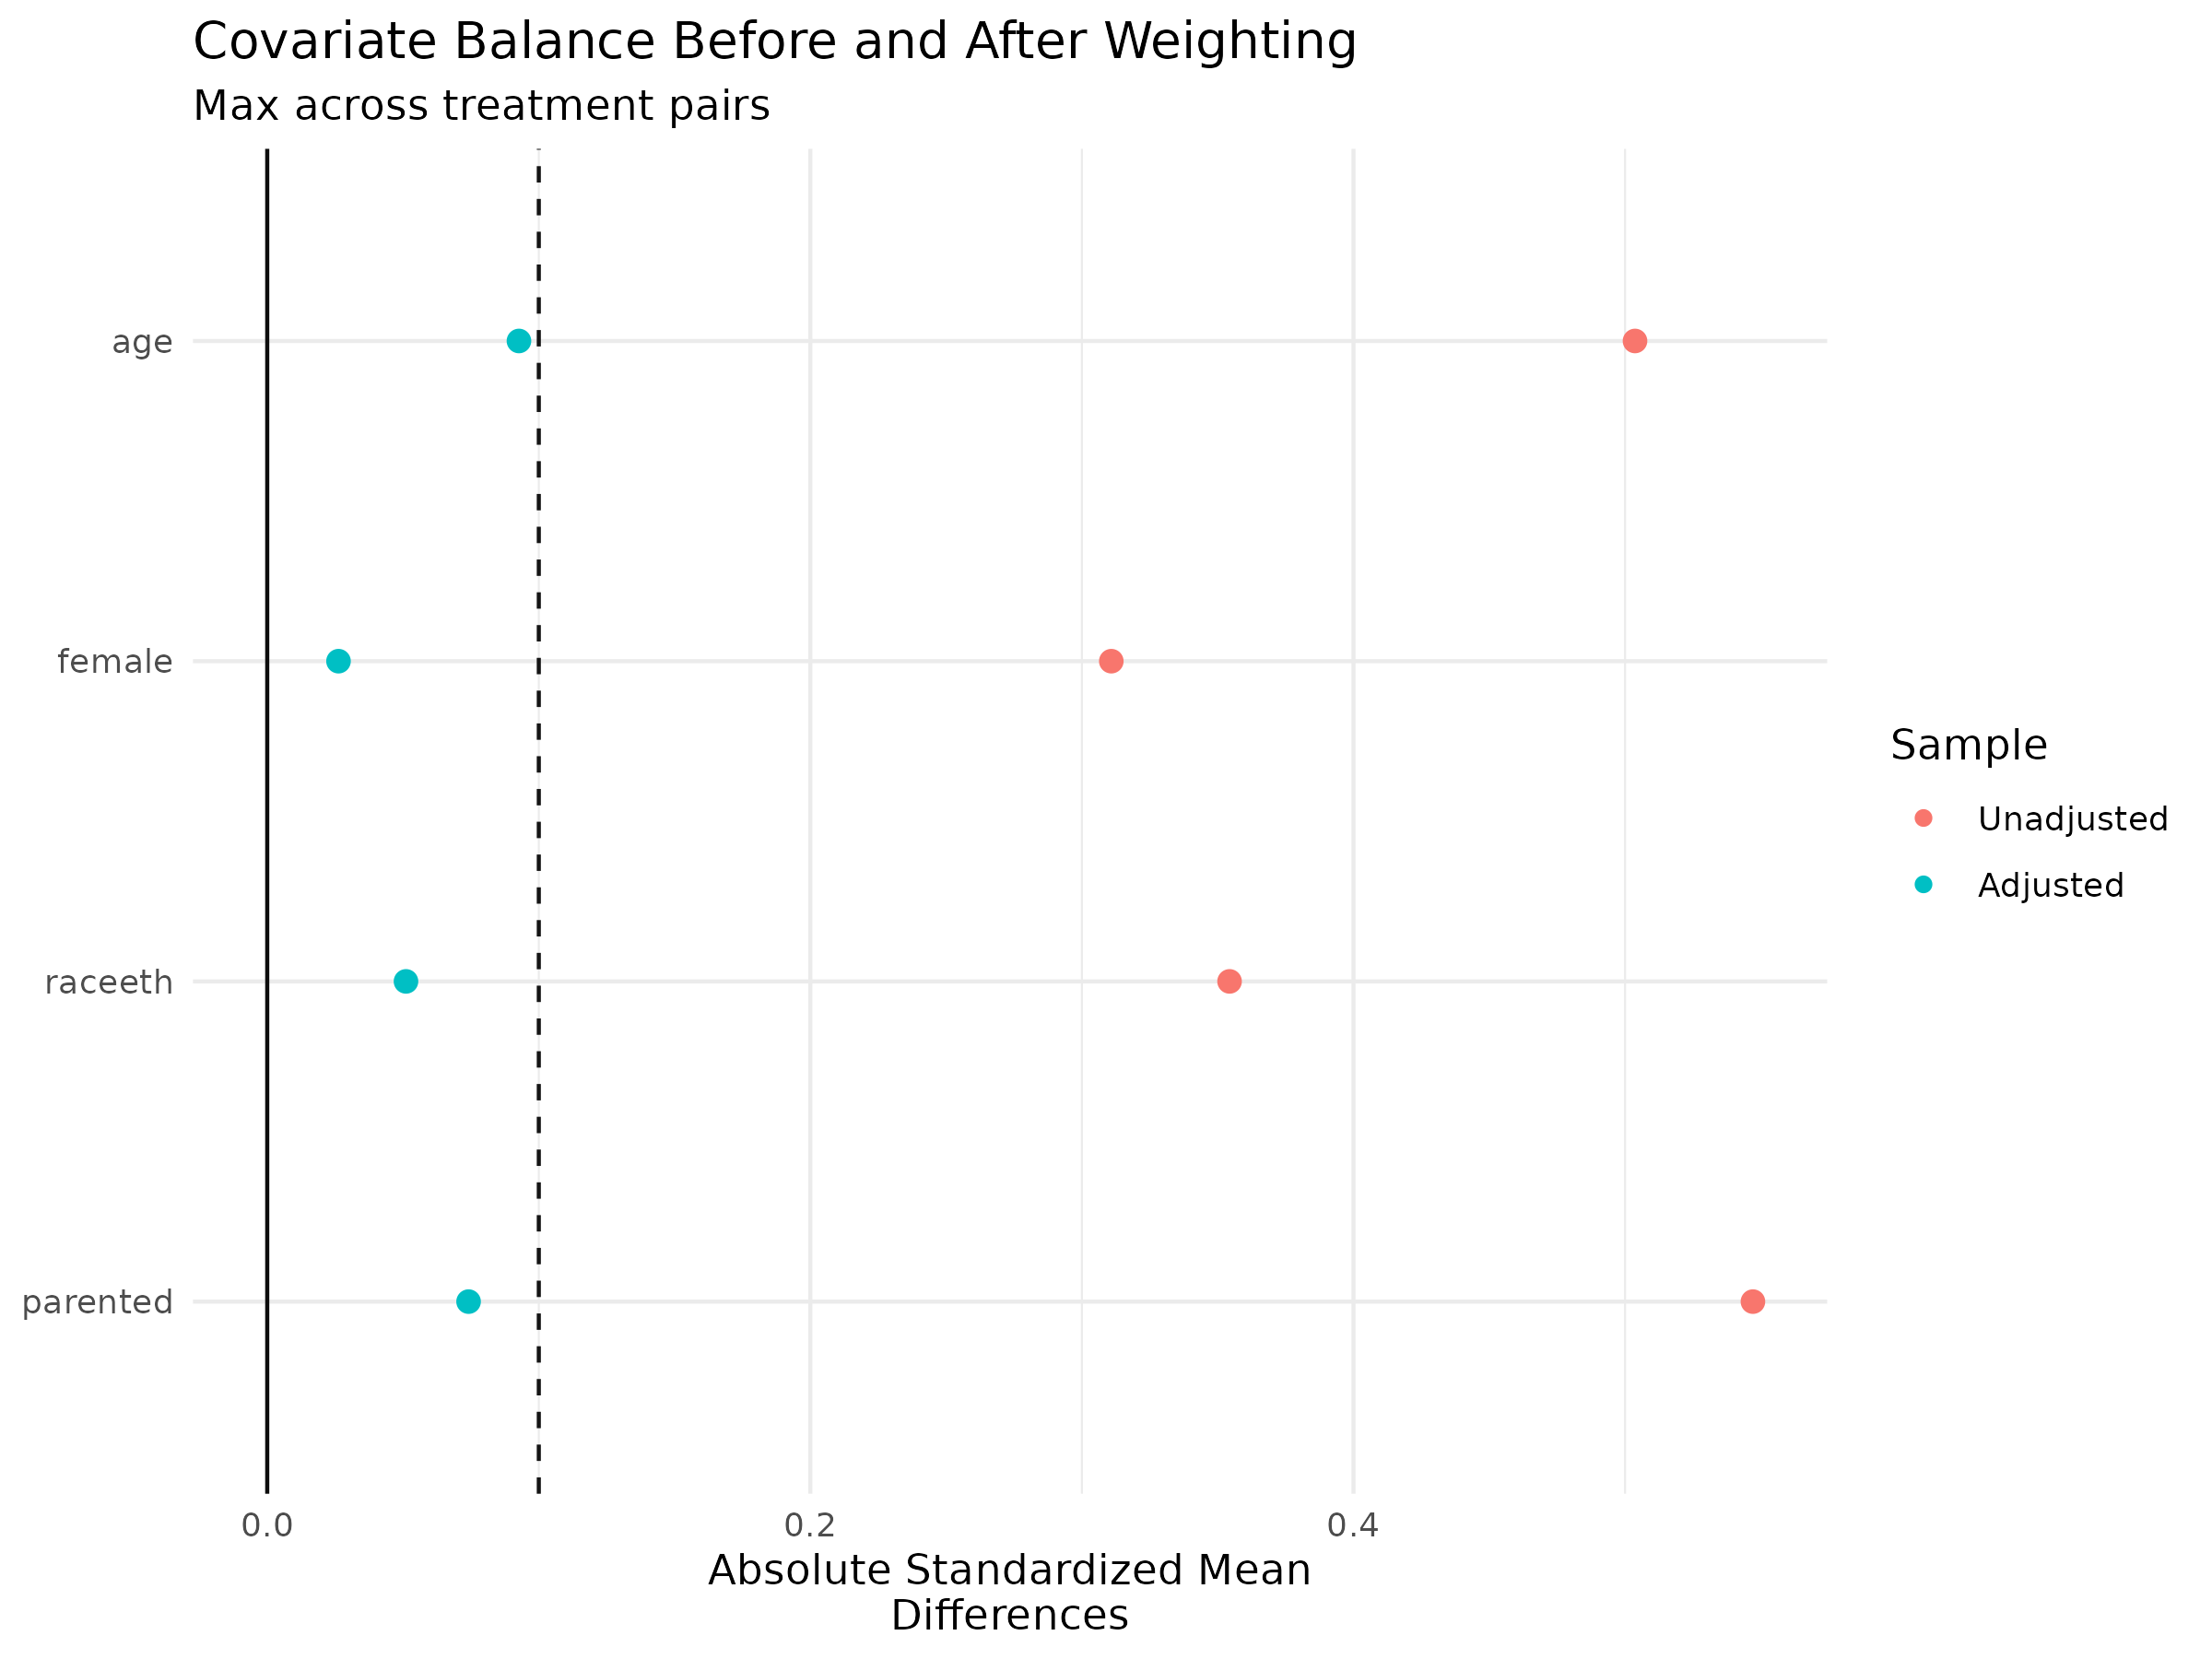
\includegraphics[width=0.8\textwidth]{figures/Figure8_CovariateBalance.png}
    \caption{Covariate Balance Across Observational Status Groups Before and After IPW Weighting. The dashed lines indicate the standard $\pm 0.10$ threshold for acceptable balance.}
    \label{fig:balance}
\end{figure}

\subsection{Counterfactual Exposure Drift in the Control Condition}
Evaluating the unexposed Control Condition allows us to observe the counterfactual drift in aesthetic judgments over repeated trials in the complete absence of cues from others. Because educational attainment is an observational attribute rather than an experimentally assigned condition, comparisons between college-educated and non-college respondents in the Control Condition may be subject to demographic confounding. To address this, we estimate a repeated-measures linear mixed model within the Control Condition ($N = 177$ respondents, $354$ observations) incorporating Inverse Probability Weighting (IPW) to balance baseline age, gender, race/ethnicity, and parental education:
\begin{equation}
\text{Taste}_{it} = \alpha_0 + \beta_1 \text{Trial}_{it} + \alpha_1 \text{College}_i + \beta_2 (\text{Trial}_{it} \times \text{College}_i) + u_i + \epsilon_{it}
\label{eq:drift_model}
\end{equation}
where respondents without a college degree serve as the reference category.

As shown in Model 1 of Table \ref{tbl:did_models}, the counterfactual exposure drift across trials for respondents without a college degree is statistically indistinguishable from zero ($\beta_1 = +0.032, SE = 0.058, t = 0.55, p = 0.582$; unweighted: $\beta_1 = 0.000, SE = 0.052, p = 1.000$). In contrast, the interaction between Trial and College degree is positive and statistically significant ($\beta_2 = +0.247, SE = 0.082, t = 3.00, p = 0.0027^{**}$; unweighted: $\beta_2 = +0.257, SE = 0.080, p = 0.0016^{**}$). Combining these parameters reveals that college-educated respondents exhibit substantial upward exposure drift ($\text{Total Drift} = +0.279, SE = 0.063, t = 4.43, p < 0.001$; unweighted: $+0.257, p < 0.001$). Thus, after balancing baseline demographic covariates, repeated exposure produces an intrinsic aesthetic appreciation specifically among respondents possessing institutionalized cultural capital, whereas non-college respondents maintain static evaluations.

\subsection{Valence Asymmetry in Difference-in-Differences Effects}
Model 2 of Table \ref{tbl:did_models} presents the primary Difference-in-Differences (DiD) estimates for the pooled sample ($N = 2,253$). In the pooled sample, average exposure drift across trials in the absence of treatment is positive ($\beta_1 = +0.107, SE = 0.052, t = 2.05, p = 0.041$). Because experimental treatments were randomly assigned, the primary specification is unweighted; an auxiliary IPW-weighted model balancing background demographics yields consistent substantive patterns (Appendix Table A.2).

\begin{table}[ht!]
\centering
\small
\caption{Linear Mixed-Effects Models of Counterfactual Exposure Drift and Difference-in-Differences Treatment Effects}
\label{tbl:did_models}
\setlength{\tabcolsep}{4.5pt}
\begin{tabular*}{\linewidth}{@{\extracolsep{\fill}}lcccc@{}}
\toprule
& \multicolumn{2}{c}{\textbf{Model 1: Control Drift Model (IPW)}} & \multicolumn{2}{c}{\textbf{Model 2: Pooled DiD Model}} \\
\cmidrule(lr){2-3} \cmidrule(lr){4-5}
\textbf{Independent Variable} & Estimate (SE) & $t$ value & Estimate (SE) & $t$ value \\
\midrule
Intercept & 4.861 (0.155) & 31.42$^{***}$ & 4.689 (0.114) & 40.99$^{***}$ \\
Trial 2 Exposure Drift ($\beta_1$) & +0.032 (0.058) & 0.55 & +0.107 (0.052) & 2.05$^{*}$ \\
College Degree Main Effect & -0.433 (0.238) & -1.82$^{\dagger}$ & \multicolumn{2}{c}{---} \\
Trial 2 $\times$ College Degree ($\beta_2$) & +0.247 (0.082) & 3.00$^{**}$ & \multicolumn{2}{c}{---} \\
\addlinespace[3pt]
\multicolumn{5}{l}{\textit{Treatment Main Effects at Baseline ($\beta_k$):}} \\
\quad Low-Status Like & \multicolumn{2}{c}{---} & +0.095 (0.145) & 0.66 \\
\quad High-Status Like & \multicolumn{2}{c}{---} & -0.039 (0.131) & -0.30 \\
\quad Low-Status Dislike & \multicolumn{2}{c}{---} & +0.068 (0.145) & 0.47 \\
\quad High-Status Dislike & \multicolumn{2}{c}{---} & +0.061 (0.131) & 0.47 \\
\quad Generalized Like & \multicolumn{2}{c}{---} & -0.172 (0.163) & -1.05 \\
\quad Generalized Dislike & \multicolumn{2}{c}{---} & +0.229 (0.163) & 1.41 \\
\addlinespace[3pt]
\multicolumn{5}{l}{\textit{Difference-in-Differences Treatment Effects ($\delta_k = \text{Trial} \times \text{Condition}$):}} \\
\quad Low-Status Like & \multicolumn{2}{c}{---} & -0.128 (0.067) & -1.93$^{\dagger}$ \\
\quad High-Status Like & \multicolumn{2}{c}{---} & +0.041 (0.060) & 0.68 \\
\quad Low-Status Dislike & \multicolumn{2}{c}{---} & +0.016 (0.066) & 0.23 \\
\quad High-Status Dislike & \multicolumn{2}{c}{---} & -0.121 (0.060) & -2.02$^{*}$ \\
\quad Generalized Like & \multicolumn{2}{c}{---} & +0.096 (0.075) & 1.29 \\
\quad Generalized Dislike & \multicolumn{2}{c}{---} & -0.125 (0.075) & -1.67$^{\dagger}$ \\
\midrule
Total College Exposure Drift & +0.279 (0.063) & 4.43$^{***}$ & \multicolumn{2}{c}{---} \\
Random Intercept Variance ($\sigma^2_u$) & \multicolumn{2}{c}{2.268} & \multicolumn{2}{c}{2.074} \\
Residual Variance ($\sigma^2_\epsilon$) & \multicolumn{2}{c}{0.592} & \multicolumn{2}{c}{0.243} \\
Observations / Individuals & \multicolumn{2}{c}{354 / 177} & \multicolumn{2}{c}{4,506 / 2,253} \\
Log Likelihood & \multicolumn{2}{c}{-487.8} & \multicolumn{2}{c}{-6,465.0} \\
\bottomrule
\end{tabular*}
\begin{minipage}{\linewidth}
\vspace{4pt}
\footnotesize
\textit{Note:} $^{\dagger}p < 0.10, ^{*}p < 0.05, ^{**}p < 0.01, ^{***}p < 0.001$. Models estimated via linear mixed-effects with random intercepts for respondents. Model 1 restricts the sample to the unexposed Control Condition ($N = 177$) and incorporates Inverse Probability Weighting (IPW) to balance baseline age, gender, race/ethnicity, and parental education between college and non-college respondents (non-college respondents serve as reference; unweighted estimates yield $\beta_1 = 0.000, p = 1.000$ and $\beta_2 = +0.257, p = 0.0016$). Model 2 estimates the primary unweighted Difference-in-Differences specification across the pooled sample ($N = 2,253$), benchmarking treatment shifts against the unexposed Control Condition.
\end{minipage}
\end{table}

The DiD results provide empirical evidence of a generalized influence effect in the pooled sample, but only for \textit{negative} judgments, suggesting that these are stronger signals than positive ones. Specifically, negative feedback suppresses the overall positive drift effect: negative evaluations from others significantly halt and reverse the positive exposure drift observed in the control condition. Exposure to High-Status Dislike leads to a statistically significant negative divergence of $\text{DiD} = -0.121$ ($SE = 0.060, t = -2.02, p = 0.043^{*}$) relative to the control condition. Generalized Dislike similarly exerts a marginally significant suppressive DiD effect of $\text{DiD} = -0.125$ ($SE = 0.075, t = -1.67, p = 0.095^{\dagger}$). Furthermore, exposure to Low-Status Likes produces a marginally significant negative DiD shift of $\text{DiD} = -0.128$ ($SE = 0.067, t = -1.93, p = 0.055^{\dagger}$).

In contrast, exposure to positive evaluations from others fails to produce statistically significant facilitative shifts relative to the control exposure drift. The DiD estimate for High-Status Like is small and statistically indistinguishable from zero ($\text{DiD} = +0.041, SE = 0.060, t = 0.68, p = 0.497$). Generalized Like similarly fails to achieve statistical significance in the pooled sample ($\text{DiD} = +0.096, SE = 0.075, t = 1.29, p = 0.198$). Exposure to Low-Status Dislike is likewise null ($\text{DiD} = +0.016, SE = 0.066, t = 0.23, p = 0.815$). Because positive evaluations from others do not reach statistical significance ($p \ge 0.10$), we cannot conclude that positive cues produce a reliable facilitative effect in the aggregate. Rather, the statistically reliable pooled influence of external information operates as an asymmetric veto: negative evaluations from others actively suppress the appreciation that emerges under repeated exposure alone.

\subsection{Stepwise Analysis: Social Influence Moderated by Education and Subjective Class Separately}
\label{sec:stepwise_models}
Before examining the four-quadrant status consistency typology, we disaggregate the analysis to inspect how educational attainment alone (College Degree vs.\ No College) and subjective social class alone (Working Class vs.\ Middle Class) moderate the experimental treatments. Figure \ref{fig:did_edu_class} presents the complete set of Difference-in-Differences estimates across all cue conditions for both dimensions, and Table \ref{tbl:did_edu_class} reports the detailed model coefficients and standard errors.

\begin{figure}[ht!]
    \centering
    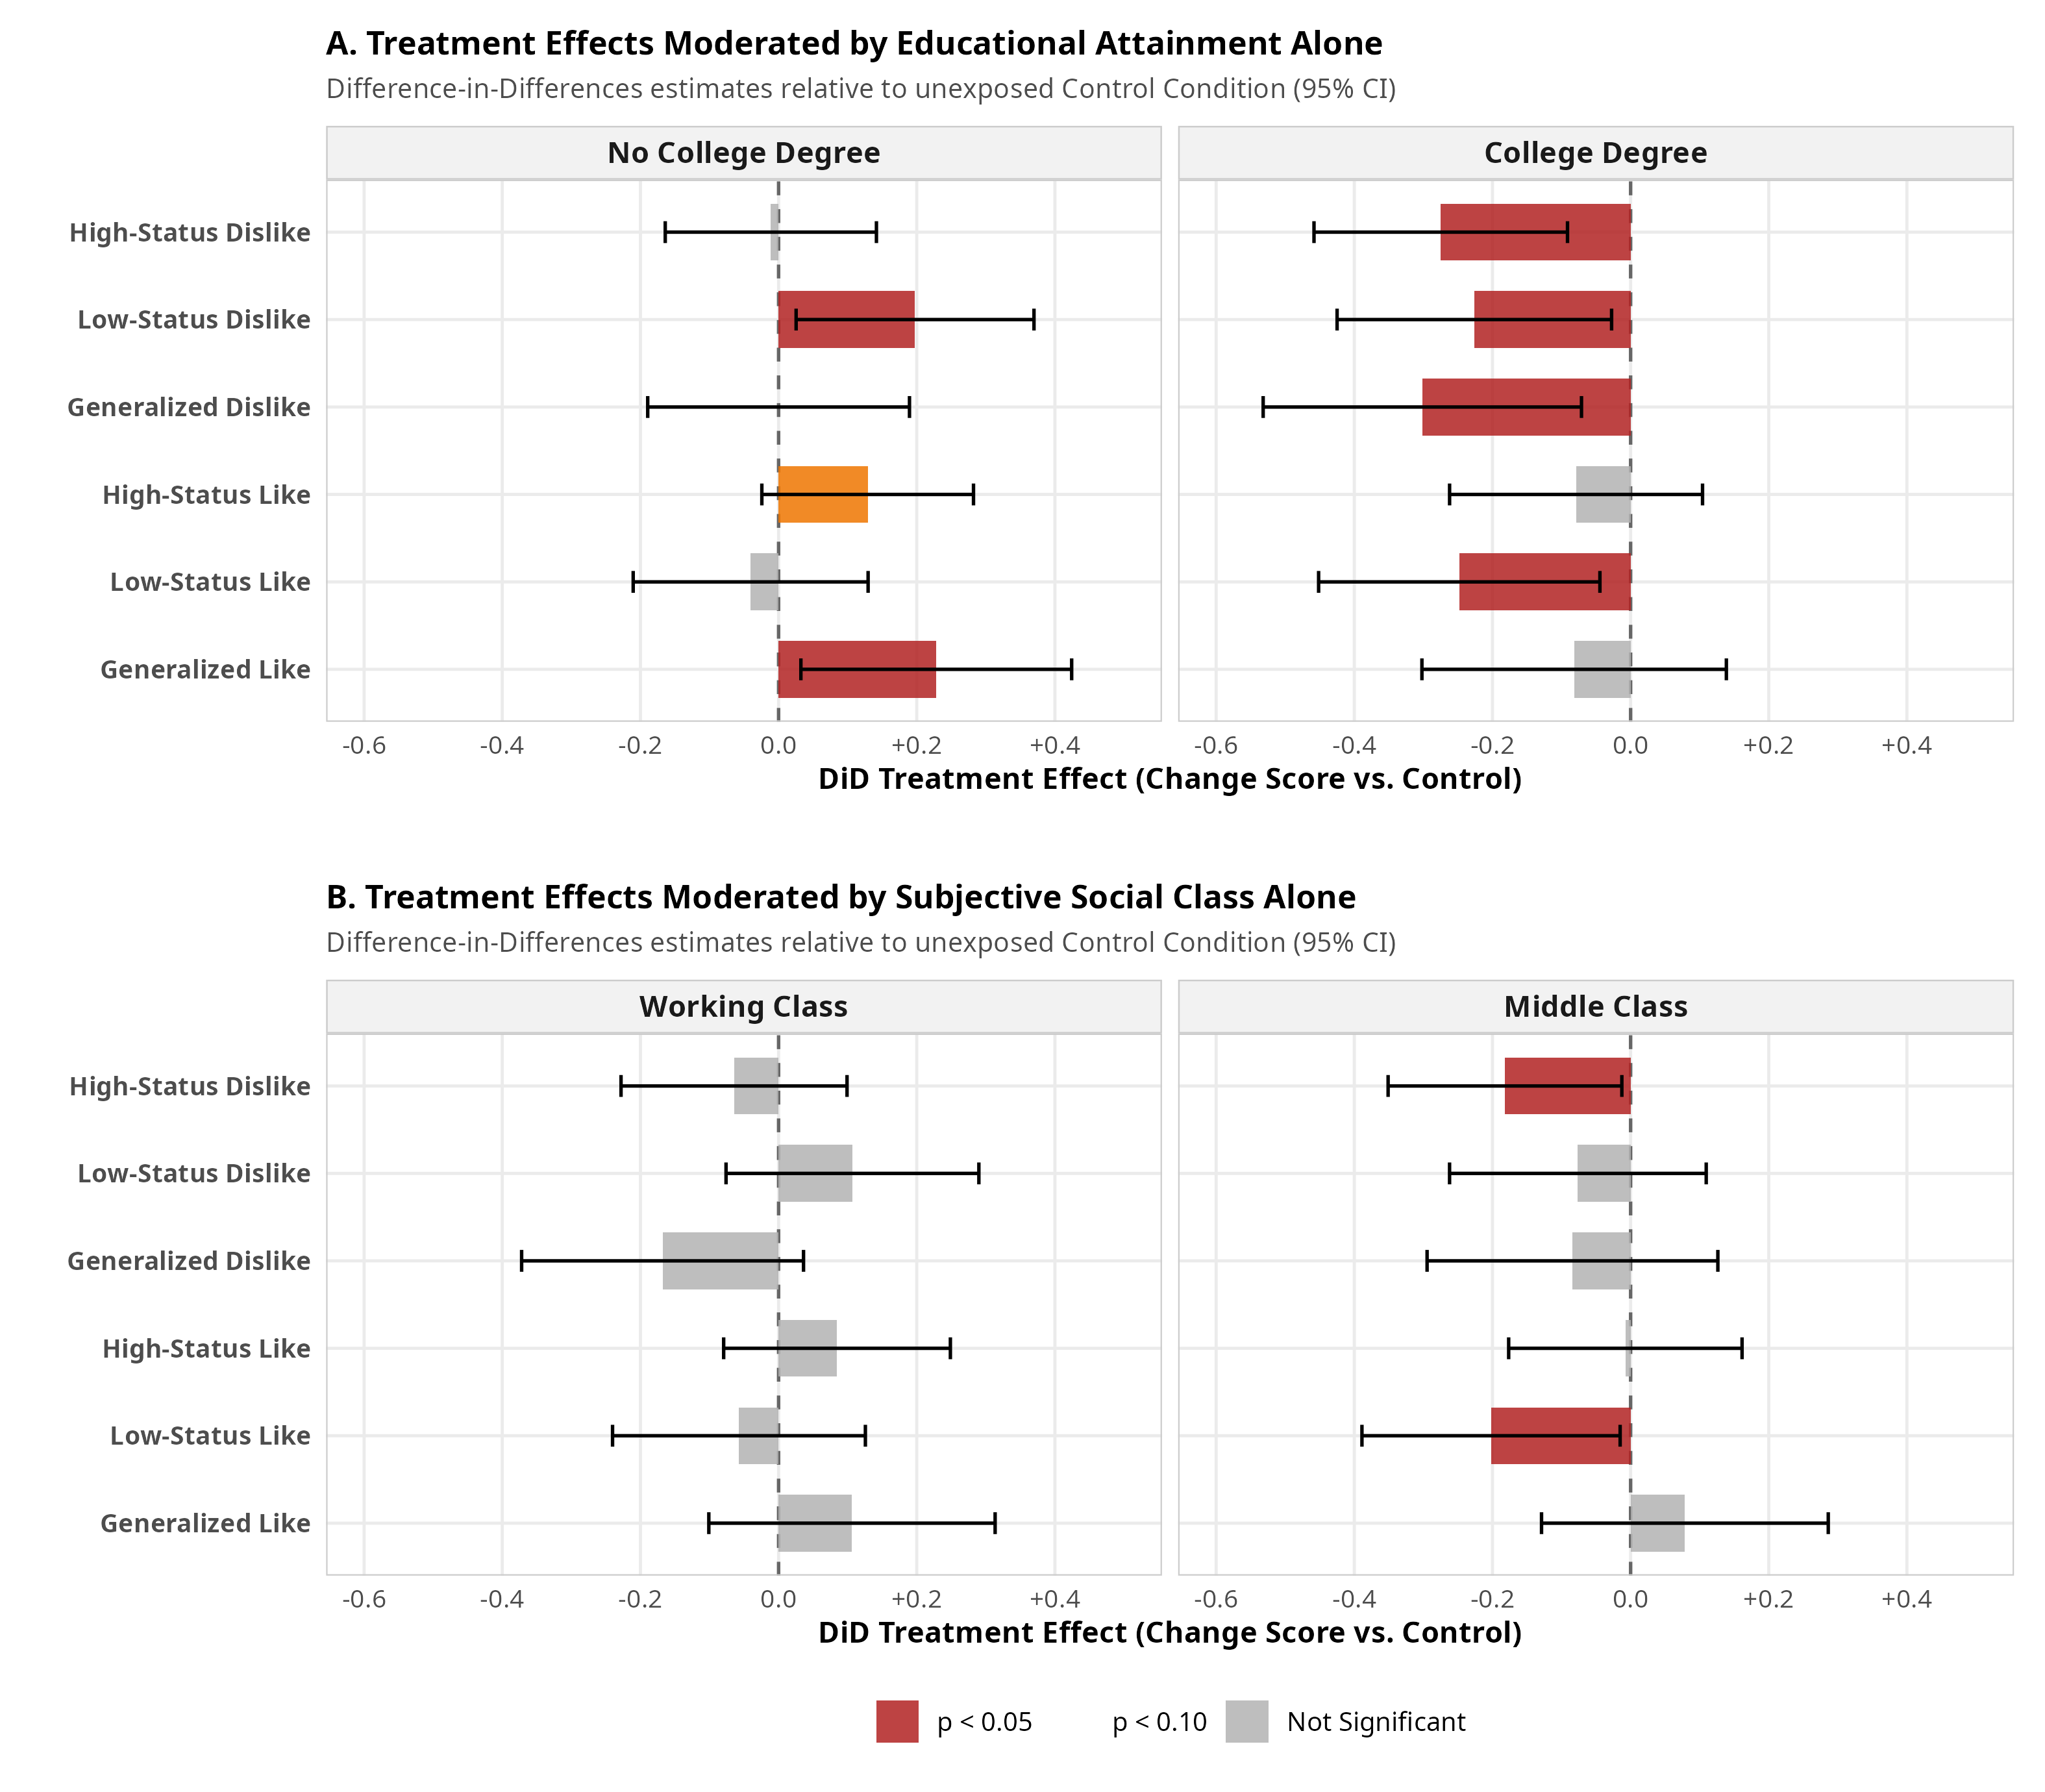
\includegraphics[width=0.92\textwidth]{figures/Figure_DiD_Edu_Class_Separate.png}
    \caption{Difference-in-Differences Treatment Effects Moderated Separately by Educational Attainment (Panel A) and Subjective Social Class (Panel B). Horizontal bars depict point estimates with 95\% confidence intervals benchmarked against the unexposed Control Condition. Colors indicate statistical significance: red ($p < 0.05$), orange ($p < 0.10$), and grey ($p \ge 0.10$).}
    \label{fig:did_edu_class}
\end{figure}

\begin{table}[ht!]
\centering
\small
\caption{Difference-in-Differences Estimates Moderated Separately by Education and Subjective Class}
\label{tbl:did_edu_class}
\setlength{\tabcolsep}{4.5pt}
\begin{tabular*}{\linewidth}{@{\extracolsep{\fill}}lcccc@{}}
\toprule
& \multicolumn{2}{c}{\textbf{Panel A: Education Alone}} & \multicolumn{2}{c}{\textbf{Panel B: Subjective Class Alone}} \\
\cmidrule(lr){2-3} \cmidrule(lr){4-5}
\textbf{Treatment Condition} & No College & College Degree & Working Class & Middle Class \\
\midrule
High-Status Dislike & -0.011 (0.078) & -0.275$^{**}$ (0.094) & -0.065 (0.083) & -0.182$^{*}$ (0.086) \\
Low-Status Dislike & +0.198$^{*}$ (0.088) & -0.226$^{*}$ (0.101) & +0.107 (0.093) & -0.076 (0.095) \\
Generalized Dislike & +0.000 (0.097) & -0.302$^{*}$ (0.118) & -0.168 (0.104) & -0.084 (0.107) \\
High-Status Like & +0.129$^{\dagger}$ (0.078) & -0.079 (0.093) & +0.085 (0.084) & -0.008 (0.086) \\
Low-Status Like & -0.040 (0.087) & -0.248$^{*}$ (0.104) & -0.057 (0.093) & -0.202$^{*}$ (0.095) \\
Generalized Like & +0.228$^{*}$ (0.100) & -0.082 (0.112) & +0.106 (0.106) & +0.079 (0.106) \\
\midrule
Control Condition Drift & -0.000 (0.069) & +0.257$^{**}$ (0.081) & +0.065 (0.072) & +0.155$^{*}$ (0.076) \\
Sample Size ($N$) & 1,340 & 913 & 1,099 & 1,154 \\
\bottomrule
\end{tabular*}
\begin{minipage}{\linewidth}
\vspace{4pt}
\footnotesize
\textit{Note:} $^{\dagger}p < 0.10, ^{*}p < 0.05, ^{**}p < 0.01, ^{***}p < 0.001$. Estimates represent Difference-in-Differences treatment contrasts relative to the unexposed Control Condition within each demographic subpopulation. Panel A estimates moderation by educational attainment alone (No College Degree vs.\ Bachelor's Degree or Higher). Panel B estimates moderation by subjective social class identification alone (Working Class vs.\ Middle Class).
\end{minipage}
\end{table}

Inspecting the separate models reveals that educational capital is the primary structural fault line governing both counterfactual baseline drift and responsiveness to external evaluations (Panel A of Figure \ref{fig:did_edu_class}). Non-college respondents show flat evaluative stability in the absence of cues ($\beta_{\text{Trial}} = 0.000, p = 1.00$). When presented with information from others, they exhibit positive shifts under Generalized Likes ($\text{DiD} = +0.228, SE = 0.100, p = 0.022^{*}$) and Low-Status Dislikes ($\text{DiD} = +0.198, SE = 0.088, p = 0.025^{*}$), while remaining largely unresponsive to high-status cues. Conversely, college-educated respondents exhibit pronounced baseline exposure drift ($\beta_{\text{Trial}} = +0.257, SE = 0.081, p = 0.016^{*}$) that is strongly curtailed by external negative cues: High-Status Dislike ($\text{DiD} = -0.275, SE = 0.094, p = 0.003^{**}$), Generalized Dislike ($\text{DiD} = -0.302, SE = 0.118, p = 0.010^{*}$), and Low-Status Dislike ($\text{DiD} = -0.226, SE = 0.101, p = 0.026^{*}$). In addition, college graduates exhibit Bourdieusian taste abandonment when exposed to Low-Status Likes ($\text{DiD} = -0.248, SE = 0.104, p = 0.017^{*}$).

By comparison, examining subjective social class in isolation (Panel B of Figure \ref{fig:did_edu_class}) produces a more diffuse picture. Self-identified working-class respondents show no statistically reliable DiD adjustments across any condition, masking substantial underlying heterogeneity. Middle-class self-identifiers display significant negative shifts under High-Status Dislike ($\text{DiD} = -0.182, SE = 0.086, p = 0.035^{*}$) and Low-Status Like ($\text{DiD} = -0.202, SE = 0.095, p = 0.034^{*}$), but these effects are attenuated relative to the education-stratified models.

Crucially, this stepwise comparison demonstrates why analyzing education and subjective class separately is insufficient. Because objective credential attainment and subjective class identification cross-cut one another—nearly 28\% of working-class self-identifiers hold college degrees, while over 28\% of middle-class identifiers do not—univariate stratification conflates status-consistent actors with status-inconsistent actors. As we show below, the apparent lack of responsiveness among ``working-class'' respondents is an artifact of aggregating non-college workers (who exhibit normative inertia) with college-educated workers (who exhibit sharp reactivity against high-status cues). Examining their four-quadrant intersection is therefore essential for isolating the distinct mechanisms of status consistency and cross-status influence.

\subsection{Status-Differentiated Influence: Testing Hypotheses 1--3}
Evaluating our status-differentiated hypotheses through the DiD framework (reported across all 24 cells in Appendix Figure \ref{fig:did_status_full} and summarized in Table \ref{tbl:hypotheses_summary}) reveals which theoretical expectations are empirically supported versus unsupported across status groups.

First, same-status alignment (\textit{Hypothesis 1}) is not supported. Hypothesis 1 predicted that individuals would align their judgments with the positive and negative evaluations of others sharing their status. When evaluated relative to the control condition counterfactual, neither high-status consistent respondents ($\text{DiD} = -0.118, SE = 0.126, p = 0.348$) nor low-status consistent respondents ($\text{DiD} = -0.110, SE = 0.132, p = 0.404$) show a statistically significant DiD shift when exposed to same-status likes. Similarly, low-status respondents exposed to same-status dislikes do not exhibit a statistically significant shift ($\text{DiD} = +0.185, SE = 0.132, p = 0.163$). Because none of these estimates achieve statistical significance ($p \ge 0.10$), the data do not support Hypothesis 1.

Second, symbolic power and upward alignment (\textit{Hypothesis 2}) is not supported for low-status consistent individuals. Hypothesis 2 predicted that low-status respondents would align with high-status evaluations. Among low-status consistent respondents (Working Class/No College), neither exposure to High-Status Likes ($\text{DiD} = +0.130, SE = 0.115, p = 0.256$) nor High-Status Dislikes ($\text{DiD} = +0.006, SE = 0.115, p = 0.959$) produces a statistically significant change. Thus, Hypothesis 2 is not supported for low-status consistent individuals. However, for status-inconsistent workers who hold a college degree (Working Class/College), exposure to High-Status Dislikes produces a statistically significant negative DiD shift of $\text{DiD} = -0.394$ ($SE = 0.119, t = -3.30, p = 0.001^{**}$), alongside a significant negative shift under Generalized Dislikes ($\text{DiD} = -0.396, SE = 0.154, p = 0.010^{*}$). This indicates that sensitivity to high-status negative evaluation is concentrated among individuals who possess institutional cultural capital but identify with the working class.

Third, cross-status reactance and taste abandonment (\textit{Hypothesis 3}) is strongly supported. Netting out the counterfactual exposure drift provides direct empirical support for Hypothesis 3. For high-status consistent respondents (Middle Class/College), exposure to Low-Status Likes (working-class others liking the painting) produces a statistically significant negative DiD divergence of $\text{DiD} = -0.296$ ($SE = 0.144, t = -2.06, p = 0.039^{*}$) relative to the control condition. Because college-educated middle-class respondents naturally drift upward by $+0.200$ under mere exposure, discovering that working-class others liked the artwork actively reverses their appreciation. High-status consistent respondents also exhibit marginal negative shifts under Generalized Dislikes ($\text{DiD} = -0.264, SE = 0.151, p = 0.081^{\dagger}$) and Low-Status Dislikes ($\text{DiD} = -0.227, SE = 0.136, p = 0.097^{\dagger}$). This confirms that high-status individuals distance their judgments from low-status endorsements, providing experimental evidence of Bourdieusian symbolic distinction.

Finally, regarding status-inconsistent positive influence, among Middle Class individuals without a college degree, exposure to Generalized Likes produces a marginally significant positive DiD shift of $\text{DiD} = +0.338$ ($SE = 0.173, t = 1.96, p = 0.050^{\dagger}$). All other conditions for this group remain statistically indistinguishable from zero ($p \ge 0.11$).

\subsection{Discrete Behavioral Choices: Inertia, Conformity, and Reactance}
While continuous change models identify average shifts across conditions, they mask non-linear behavioral choices where opposing individual movements cancel each other out in the aggregate. For instance, an average shift close to zero could reflect complete evaluative rigidity, or it could reflect equal proportions of respondents conforming and reacting in opposite directions. To examine these discrete underlying choices, we categorize responses into three mutually exclusive behaviors: \textit{Stay} ($\Delta = 0$, maintaining one's initial evaluation), \textit{Conform} (moving in the direction of others' evaluation), and \textit{React} (moving in the opposite direction of others' evaluation). 

Figure \ref{fig:multinom} presents the Average Marginal Effects (AME) on the probability of each behavioral choice from an IPW-weighted multinomial logistic regression, benchmarked against the reference group of Working Class respondents without a college degree. In the baseline reference group, the predicted probabilities are $74.4\%$ for staying, $13.6\%$ for conforming, and $12.0\%$ for reacting.

\begin{figure}[ht!]
    \centering
    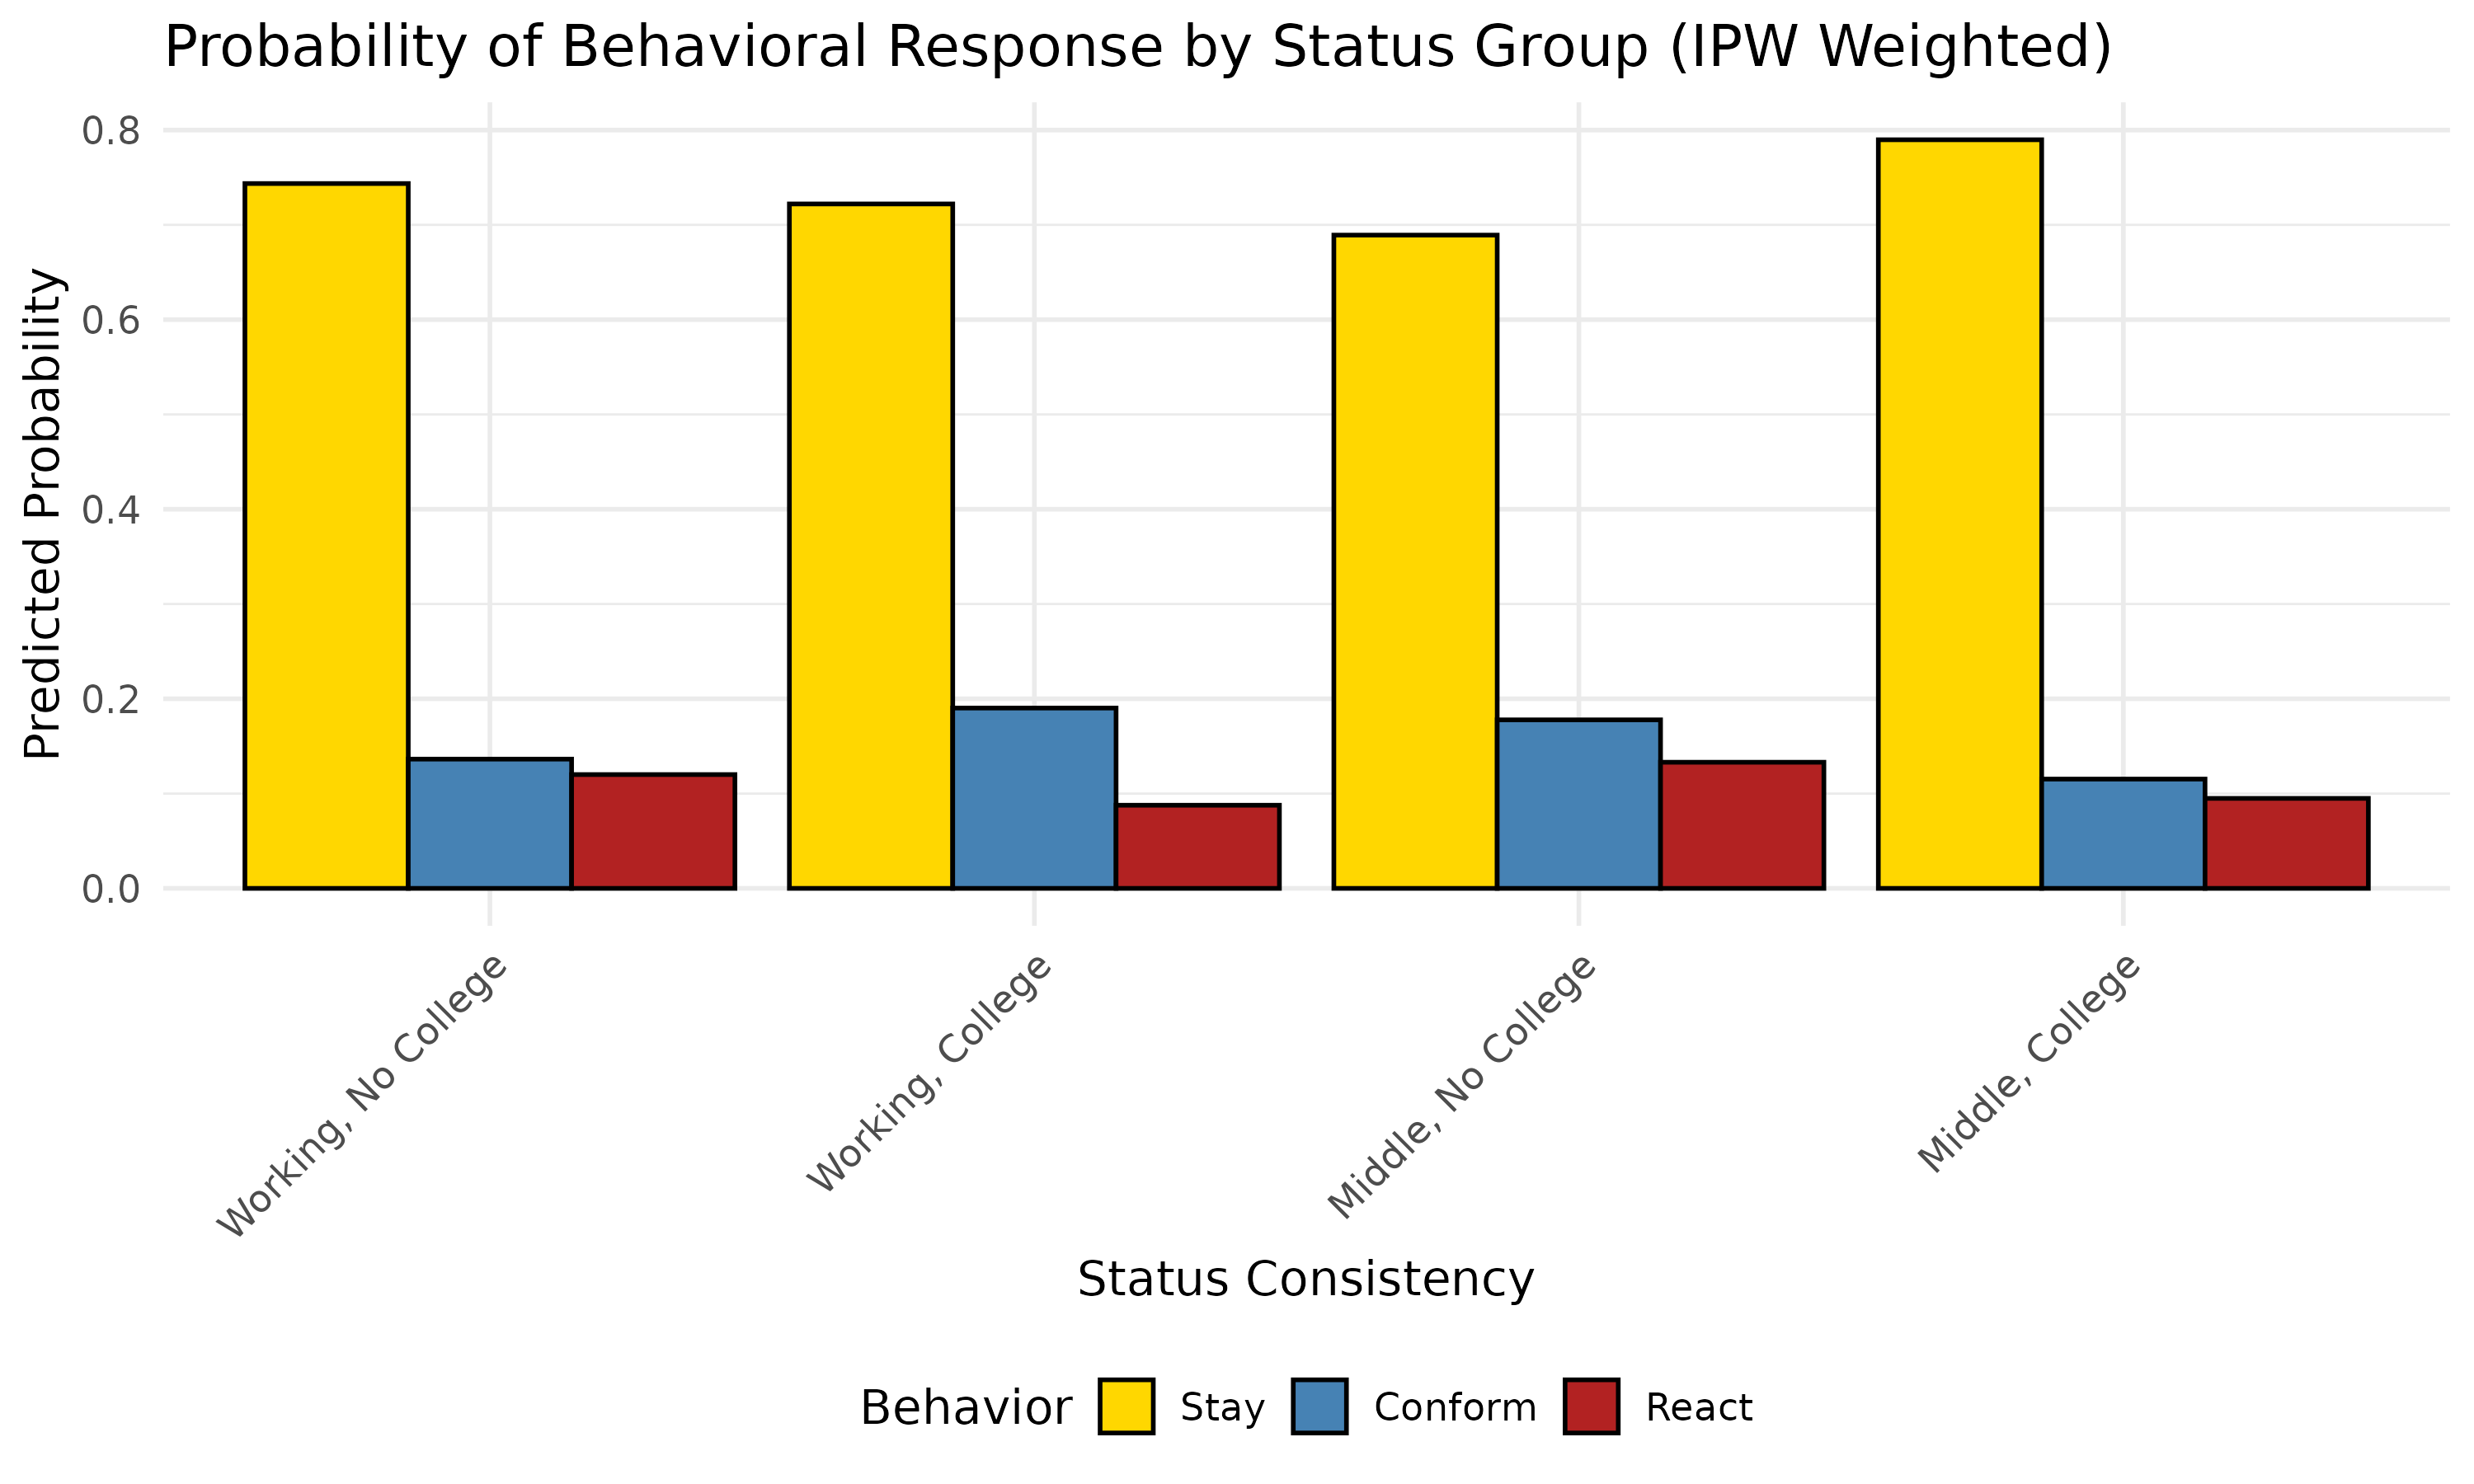
\includegraphics[width=0.95\textwidth]{figures/Figure7_MultinomialBehavior.png}
    \caption{Average Marginal Effects on Behavioral Choices (Stay, Conform, React) Across Status Consistency Groups. Horizontal bars indicate differences in choice probability relative to the baseline reference category (Working Class, No College), with 95\% confidence intervals. Colors indicate statistical significance: red ($p < 0.05$) and grey ($p \ge 0.10$).}
    \label{fig:multinom}
\end{figure}

The marginal effects provide compelling empirical confirmation of \textit{Hypothesis 4}, while providing new insights into the social psychology of status inconsistency. First, in terms of evaluative stability (Panel A: Stay), structural status consistency acts as the primary anchor of aesthetic confidence and inertia. Middle Class individuals with a college degree are significantly more likely to maintain their initial judgment compared to non-college workers ($\text{AME} = +0.046, SE = 0.013, z = 3.64, p < 0.001$), reaching an overall stay rate of $79.0\%$. In sharp contrast, status-inconsistent individuals without a college degree exhibit significantly lower stability ($\text{AME} = -0.054, SE = 0.013, z = -4.05, p < 0.001$), with their stay rate falling to $65.5\%$. College-educated workers also display attenuated stability ($\text{AME} = -0.022, p = 0.105$, stay rate $68.2\%$). This shows that evaluative inertia is not a simple linear function of high status; rather, both high-consistent (Middle/College) and low-consistent (Working/No College) individuals occupy unambiguous positions within the social structure that foster normative certainty, whereas status inconsistency breeds evaluative fluidity.

Second, in terms of conformity (Panel B), status inconsistency emerges as the primary driver of susceptibility to external social influence. Both status-inconsistent groups display large, highly significant increases in the probability of conforming to others' judgments. Working Class individuals with a college degree are $+5.4\%$ more likely to conform relative to the reference group ($\text{AME} = +0.054, SE = 0.011, z = 4.86, p < 0.001$), and Middle Class individuals without college are $+4.1\%$ more likely to conform ($\text{AME} = +0.041, SE = 0.011, z = 3.82, p < 0.001$). In stark contrast, high-status consistent individuals are significantly less likely to conform ($\text{AME} = -0.021, SE = 0.010, z = -2.11, p = 0.035$). This shows that when actors occupy contradictory locations in social space—possessing formal educational credentials while identifying as working class, or claiming middle-class status without institutional degrees—they experience evaluative cross-pressures and cognitive ambiguity that heighten their inclination to align with external social signals.

Finally, in terms of oppositional reactance (Panel C), behavioral divergence is heavily structured by educational capital. Both college-educated groups are significantly less likely to move away from others' judgments compared to non-college workers: Working Class respondents with a college degree are $-3.2\%$ less likely to react ($\text{AME} = -0.032, SE = 0.009, z = -3.54, p < 0.001$), and Middle Class college graduates are $-2.5\%$ less likely to react ($\text{AME} = -0.025, SE = 0.009, z = -2.70, p = 0.007$). Meanwhile, Middle Class individuals without college do not differ significantly from working-class peers ($\text{AME} = +0.013, p = 0.191$). This shows that oppositional reactance against external cues is concentrated among individuals without a college education, whereas institutionalized cultural capital acts as an inhibitor of oppositional defiance.

To confirm that these behavioral dynamics are specifically driven by status-laden social cues rather than generic feedback about others' opinions, we re-estimated the multinomial model excluding the two Taste-Only conditions ($N = 1,870$). As displayed in Appendix Figure \ref{fig:sens_multinom}, the results are virtually identical: structural status consistency continues to anchor evaluative inertia (Middle Class with College: $+4.8\%, p < 0.001$), status inconsistency heightens conformity (Working Class with College: $+6.0\%, p < 0.001$; Middle Class without College: $+4.3\%, p < 0.001$), and oppositional reactance remains concentrated among non-college workers ($-3.0\%$ and $-2.1\%$ for college-educated groups, $p < 0.05$). Netting out generic popularity cues therefore confirms that status consistency uniquely structures discrete behavioral responses to social influence.

\section{Discussion}

\subsection{Summary of Key Results}
In this study, we investigated how access to others' aesthetic evaluations causally influences individual taste judgments in real time. Using a national survey experiment with a Difference-in-Differences design and inverse probability weighting, we resolved several ambiguities present in observational literature. Table \ref{tbl:hypotheses_summary} provides a systematic overview of our focal hypotheses, the empirical DiD point estimates, and the resulting empirical verdicts.

\begin{table}[ht!]
\centering
\small
\caption{Summary of Hypotheses, Difference-in-Differences Estimates, and Empirical Verdicts}
\label{tbl:hypotheses_summary}
\setlength{\tabcolsep}{4.5pt}
\begin{tabular*}{\linewidth}{@{\extracolsep{\fill}}lp{5.2cm}cc@{}}
\toprule
\textbf{Hypothesis / Mechanism} & \textbf{Theoretical Expectation} & \textbf{Empirical DiD Estimate / Statistic} & \textbf{Empirical Verdict} \\
\midrule
\textit{Mere Exposure Drift (Control)} & Upward drift in evaluation across repeated trials without external social cues & $\beta_1 = +0.107$ ($p = 0.041^{*}$) & Supported ($p < 0.05$) \\
\addlinespace[3pt]
\textit{Valence Asymmetry} & Negative cues from others halt exposure drift; positive cues facilitate drift & High-Status Dislike: $\text{DiD} = -0.121$ ($p = 0.043^{*}$); Generalized Dislike: $\text{DiD} = -0.125$ ($p = 0.095^{\dagger}$); Positive cues: null ($p \ge 0.198$) & Supported ($p < 0.05$) \\
\addlinespace[3pt]
\textit{Hypothesis 1: Same-Status Alignment} & Individuals align judgments with aggregate evaluations of others sharing their status & High-status like: $\text{DiD} = -0.118$ ($p = 0.348$); Low-status like: $\text{DiD} = -0.110$ ($p = 0.404$) & Not Supported ($p \ge 0.10$) \\
\addlinespace[3pt]
\textit{Hypothesis 2: Symbolic Power} & Lower-status individuals align judgments with high-status others & Low-status consistent like: $\text{DiD} = +0.130$ ($p = 0.256$); Working/College dislike: $\text{DiD} = -0.394$ ($p = 0.001^{**}$) & Not Supported for Low-Status Consistent ($p \ge 0.10$) \\
\addlinespace[3pt]
\textit{Hypothesis 3: Cross-Status Reactance} & Individuals distance judgments from outgroup evaluations & High-status exposed to Low-Status Like: $\text{DiD} = -0.296$ ($p = 0.039^{*}$); Low-Status Dislike: $\text{DiD} = -0.227$ ($p = 0.097^{\dagger}$) & Supported ($p < 0.05$) \\
\addlinespace[3pt]
\textit{Hypothesis 4: Status Consistency Inertia} & Consistent status profiles exhibit higher stability (``staying'') than inconsistent profiles & Stay rates: 79.0\% (Middle/College) \& 74.4\% (Working/No College) vs.\ 65.5\% \& 68.2\% for inconsistent groups & Supported ($p < 0.001$) \\
\bottomrule
\end{tabular*}
\begin{minipage}{\linewidth}
\vspace{4pt}
\footnotesize
\textit{Note:} Difference-in-Differences estimates benchmark treatment shifts against the unexposed Control Condition. Status-subgroup estimates and behavioral models incorporate Inverse Probability Weighting (IPW) on age, gender, race/ethnicity, and parental education.
\end{minipage}
\end{table}

As summarized in Table \ref{tbl:hypotheses_summary}, the DiD framework clarifies which classic sociological intuitions withstand experimental scrutiny. First, we established that repeated evaluation produces a positive exposure drift, but this drift is contingent on educational capital: college-educated individuals experience an intrinsic upward appreciation upon second exposure ($\beta_1 = +0.257, p = 0.016$), whereas non-college individuals do not ($\beta_1 = 0.000, p = 1.00$). 

Second, our findings show strong empirical evidence for \textit{valence asymmetry}. In the pooled sample, negative evaluations from others and low-status endorsements produce statistically reliable suppressive shifts relative to the control condition ($p < 0.05$ to $p < 0.10$), actively halting exposure drift. In contrast, positive evaluations from others failed to produce statistically significant facilitative shifts in the aggregate ($p \ge 0.10$), indicating that cultural distastes and out-group endorsements exert a far more dependable veto on aesthetic appreciation than positive cues from others exert on facilitation.

Third, the DiD framework reveals that two widely cited mechanisms—same-status alignment (\textit{Hypothesis 1}) and upward cultural goodwill by low-status actors (\textit{Hypothesis 2})—are not supported once counterfactual exposure drift is accounted for. For low-status consistent individuals, exposure to same-status likes ($\text{DiD} = -0.110, p = 0.404$) and high-status likes ($\text{DiD} = +0.130, p = 0.256$) remain statistically indistinguishable from zero. Instead, the primary status-driven dynamic is cross-status reactance (\textit{Hypothesis 3}): high-status consistent respondents exposed to low-status likes exhibit a statistically significant negative divergence ($\text{DiD} = -0.296, p = 0.039$), providing clean experimental evidence of Bourdieusian symbolic distinction and taste abandonment.

Finally, discrete behavioral modeling provides robust confirmation of \textit{Hypothesis 4}. Aesthetic stability (``staying'') is governed by structural status consistency rather than high status alone: both high-consistent and low-consistent individuals exhibit the highest inertia, whereas status-inconsistent individuals display heightened fluidity and conformity.

\subsection{Limitations and Suggestions for Future Work}
Several limitations of this study suggest directions for future research. In terms of operationalization and measurement, our experiment relied on a single cultural stimulus—Whistler's \textit{Nocturne}—selected for its high baseline variance. Future studies should examine whether social influence dynamics operate similarly across abstract, figurative, and commercial cultural forms.

Regarding threats to causal inference and contextual confounding, while our design randomized information about others, respondent status locations were observational. Although inverse probability weighting balanced observed demographic covariates, unmeasured psychological dispositions could contribute to status-group differences. Future research using laboratory status induction could provide complementary evidence.

Third, our study examined unidirectional influence from aggregate fictional others to individuals. In everyday life, cultural influence operates bidirectionally within evolving social networks. Investigating how reciprocal feedback loops shape aesthetic consensus represents an important next step.

Fourth, regarding temporal granularity, our experiment measured short-term evaluative shifts over the course of a survey session. Longitudinal studies tracking whether experimentally induced taste shifts persist over weeks or months would help determine the durability of these social influence effects.

Finally, in terms of institutional scope conditions, our sample was recruited through a quota-matched online panel of U.S. adults. While providing greater demographic diversity than student subject pools, cross-national replications are needed to assess how national cultural institutions shape status distinction and conformity.

\subsection{Implications: Status Consistency and Evaluative Fluidity}
Our findings carry broad implications for sociological theories of taste and stratification. Classic cultural sociology has often framed aesthetic boundary work in vertical terms: high-status actors use exclusive tastes to mark distinction, while lower-status actors display cultural goodwill. Our results qualify this model by showing that cultural influence is bounded by valence asymmetry and structural consistency.

Most importantly, our analysis highlights status consistency as a neglected driver of aesthetic orientations. Status-consistent individuals—both high and low—display high evaluative stability, anchored in unambiguous structural locations. In contrast, status-inconsistent individuals experience normative cross-pressures that produce evaluative fluidity. By examining how structural consistency interacts with external social signals, cultural sociology can move beyond static homophily toward dynamic, interactional models of aesthetic judgment.

\bibliographystyle{apalike}
\bibliography{references}

\newpage
\appendix

\section{Statistical Power and Minimum Detectable Effect (MDE) Analysis}
\label{sec:appendix_power_mde}

To rigorously evaluate the statistical precision and empirical detection boundaries of the study, we conducted a formal ex-post Minimum Detectable Effect (MDE) analysis \citep{bloom1995minimum}. Methodological scholarship has established that retrospective or ``post-hoc'' power calculations based on observed effect sizes and sample estimates are fundamentally flawed and uninformative, functioning merely as a tautological transformation of the observed $p$-value \citep{gelman2014beyond, hoenig2001abuse}. By contrast, an ex-post MDE analysis answers a principled design question: given the achieved cell sample sizes and the empirical variance structure of the repeated-measures data, what is the smallest true population effect size that the research design was adequately powered (at 80\% or 90\% power, two-tailed $\alpha = 0.05$) to detect?

In a repeated-measures Difference-in-Differences (DiD) framework where each respondent $i$ provides an initial pre-treatment aesthetic rating ($Y_{i1}$) and a post-treatment evaluation ($Y_{i2}$) on a 7-point Likert scale, the standard error of the change score $\Delta Y_i = Y_{i2} - Y_{i1}$ depends directly on the test-retest correlation $\rho$ between trials:
\begin{equation}
\sigma_{\Delta} = \sqrt{\sigma_1^2 + \sigma_2^2 - 2 \rho \sigma_1 \sigma_2}
\end{equation}
When the test-retest correlation is high, the within-subject differencing cancels out stable individual-level evaluative variance, yielding a change score standard deviation substantially smaller than the cross-sectional baseline standard deviation ($\sigma_{\Delta} \ll \sigma_1$). In our survey sample, aesthetic judgments exhibit strong stability across repeated trials ($r = 0.8945$, with $\sigma_1 = 1.500$ and $\sigma_2 = 1.548$), yielding an empirical change score standard deviation of $\sigma_{\Delta} = 0.702$. This within-subject autocorrelation reduces the standard error of treatment comparisons by more than 50\% relative to an independent post-test design without pre-treatment baselines.

For a two-sample Difference-in-Differences comparison between a treatment condition of size $N_T$ and the unexposed Control Condition of size $N_C$, the standard error is:
\begin{equation}
SE_{\text{DiD}} = \sigma_{\Delta} \sqrt{\frac{1}{N_T} + \frac{1}{N_C}}
\end{equation}
The Minimum Detectable Effect at significance level $\alpha$ (two-tailed) and statistical power $1 - \beta$ is calculated as:
\begin{equation}
\text{MDE}_{\text{raw}} = (z_{1 - \alpha/2} + z_{1 - \beta}) \times SE_{\text{DiD}}
\end{equation}
where $z_{0.975} = 1.960$ for $\alpha = 0.05$, $z_{0.80} = 0.842$ for 80\% power (multiplier $= 2.802$), and $z_{0.90} = 1.282$ for 90\% power (multiplier $= 3.242$). To facilitate comparison across studies and psychological benchmarks, effect sizes are expressed both in raw 7-point Likert scale units ($\text{MDE}_{\text{raw}}$) and as standardized effect sizes relative to baseline variance, Cohen's $d = \text{MDE}_{\text{raw}} / \sigma_1$ \citep{cohen1988statistical}.

Table \ref{tbl:mde_analysis} presents the complete MDE calculations across all analytical tiers of the experimental design, and Figure \ref{fig:mde_curves} visualizes the theoretical precision curves alongside the empirical thresholds achieved in this study.

\begin{table}[ht!]
\centering
\small
\caption{Ex-Post Minimum Detectable Effect (MDE) Analysis Across Experimental Specifications}
\label{tbl:mde_analysis}
\setlength{\tabcolsep}{5.5pt}
\begin{tabular*}{\linewidth}{@{\extracolsep{\fill}}lccccccc@{}}
\toprule
& & & & \multicolumn{2}{c}{\textbf{80\% Power}} & \multicolumn{2}{c}{\textbf{90\% Power}} \\
\cmidrule(lr){5-6} \cmidrule(lr){7-8}
\textbf{Model Specification / Level} & $N_T$ & $N_C$ & $SE$ & $\text{MDE}_{\text{raw}}$ & Cohen's $d$ & $\text{MDE}_{\text{raw}}$ & Cohen's $d$ \\
\midrule
\multicolumn{8}{l}{\textit{Panel A: Within-Subject Exposure Drift (Paired Comparison)}} \\[2pt]
Full Sample Drift & 2,253 & --- & 0.015 & 0.041 & 0.028 & 0.048 & 0.032 \\
Control Condition Drift & 177 & --- & 0.053 & 0.148 & 0.099 & 0.171 & 0.114 \\
\addlinespace[4pt]
\multicolumn{8}{l}{\textit{Panel B: Pooled Difference-in-Differences Contrasts (vs. Control $N_C=177$)}} \\[2pt]
Taste-Only Conditions & 172 & 177 & 0.075 & 0.210 & 0.140 & 0.244 & 0.162 \\
Single Status Conditions & 290 & 177 & 0.067 & 0.188 & 0.125 & 0.217 & 0.145 \\
Pooled High-Status Conditions & 575 & 177 & 0.060 & 0.169 & 0.113 & 0.196 & 0.130 \\
\addlinespace[4pt]
\multicolumn{8}{l}{\textit{Panel C: Subgroup DiD Contrasts Within Status Consistency Quadrants}} \\[2pt]
Working Class, No College & 60--214 & 70 & 0.108 & 0.304 & 0.203 & 0.352 & 0.234 \\
Middle Class, College & 51--164 & 51 & 0.124 & 0.347 & 0.231 & 0.401 & 0.267 \\
Middle Class, No College & 32--146 & 33 & 0.150 & 0.421 & 0.281 & 0.487 & 0.325 \\
Working Class, College & 16--72 & 23 & 0.186 & 0.522 & 0.348 & 0.604 & 0.403 \\
\bottomrule
\end{tabular*}
\begin{minipage}{\linewidth}
\vspace{4pt}
\footnotesize
\textit{Note:} Minimum Detectable Effects (MDE) are calculated assuming a two-tailed $\alpha = 0.05$ with standard statistical power thresholds of $80\%$ ($z = 2.802$) and $90\%$ ($z = 3.242$). Calculations incorporate the empirical test-retest correlation across repeated trials ($r = 0.8945$, yielding $\sigma_{\Delta} = 0.702$ relative to baseline $\sigma_1 = 1.500$). $\text{MDE}_{\text{raw}}$ is expressed in units of the 7-point aesthetic rating scale; Cohen's $d = \text{MDE}_{\text{raw}} / \sigma_1$. In Panel C, $N_T$ indicates the range of treatment cell sizes across specific cue conditions, and reported $SE$ and MDE values correspond to median cell sizes.
\end{minipage}
\end{table}

\begin{figure}[ht!]
    \centering
    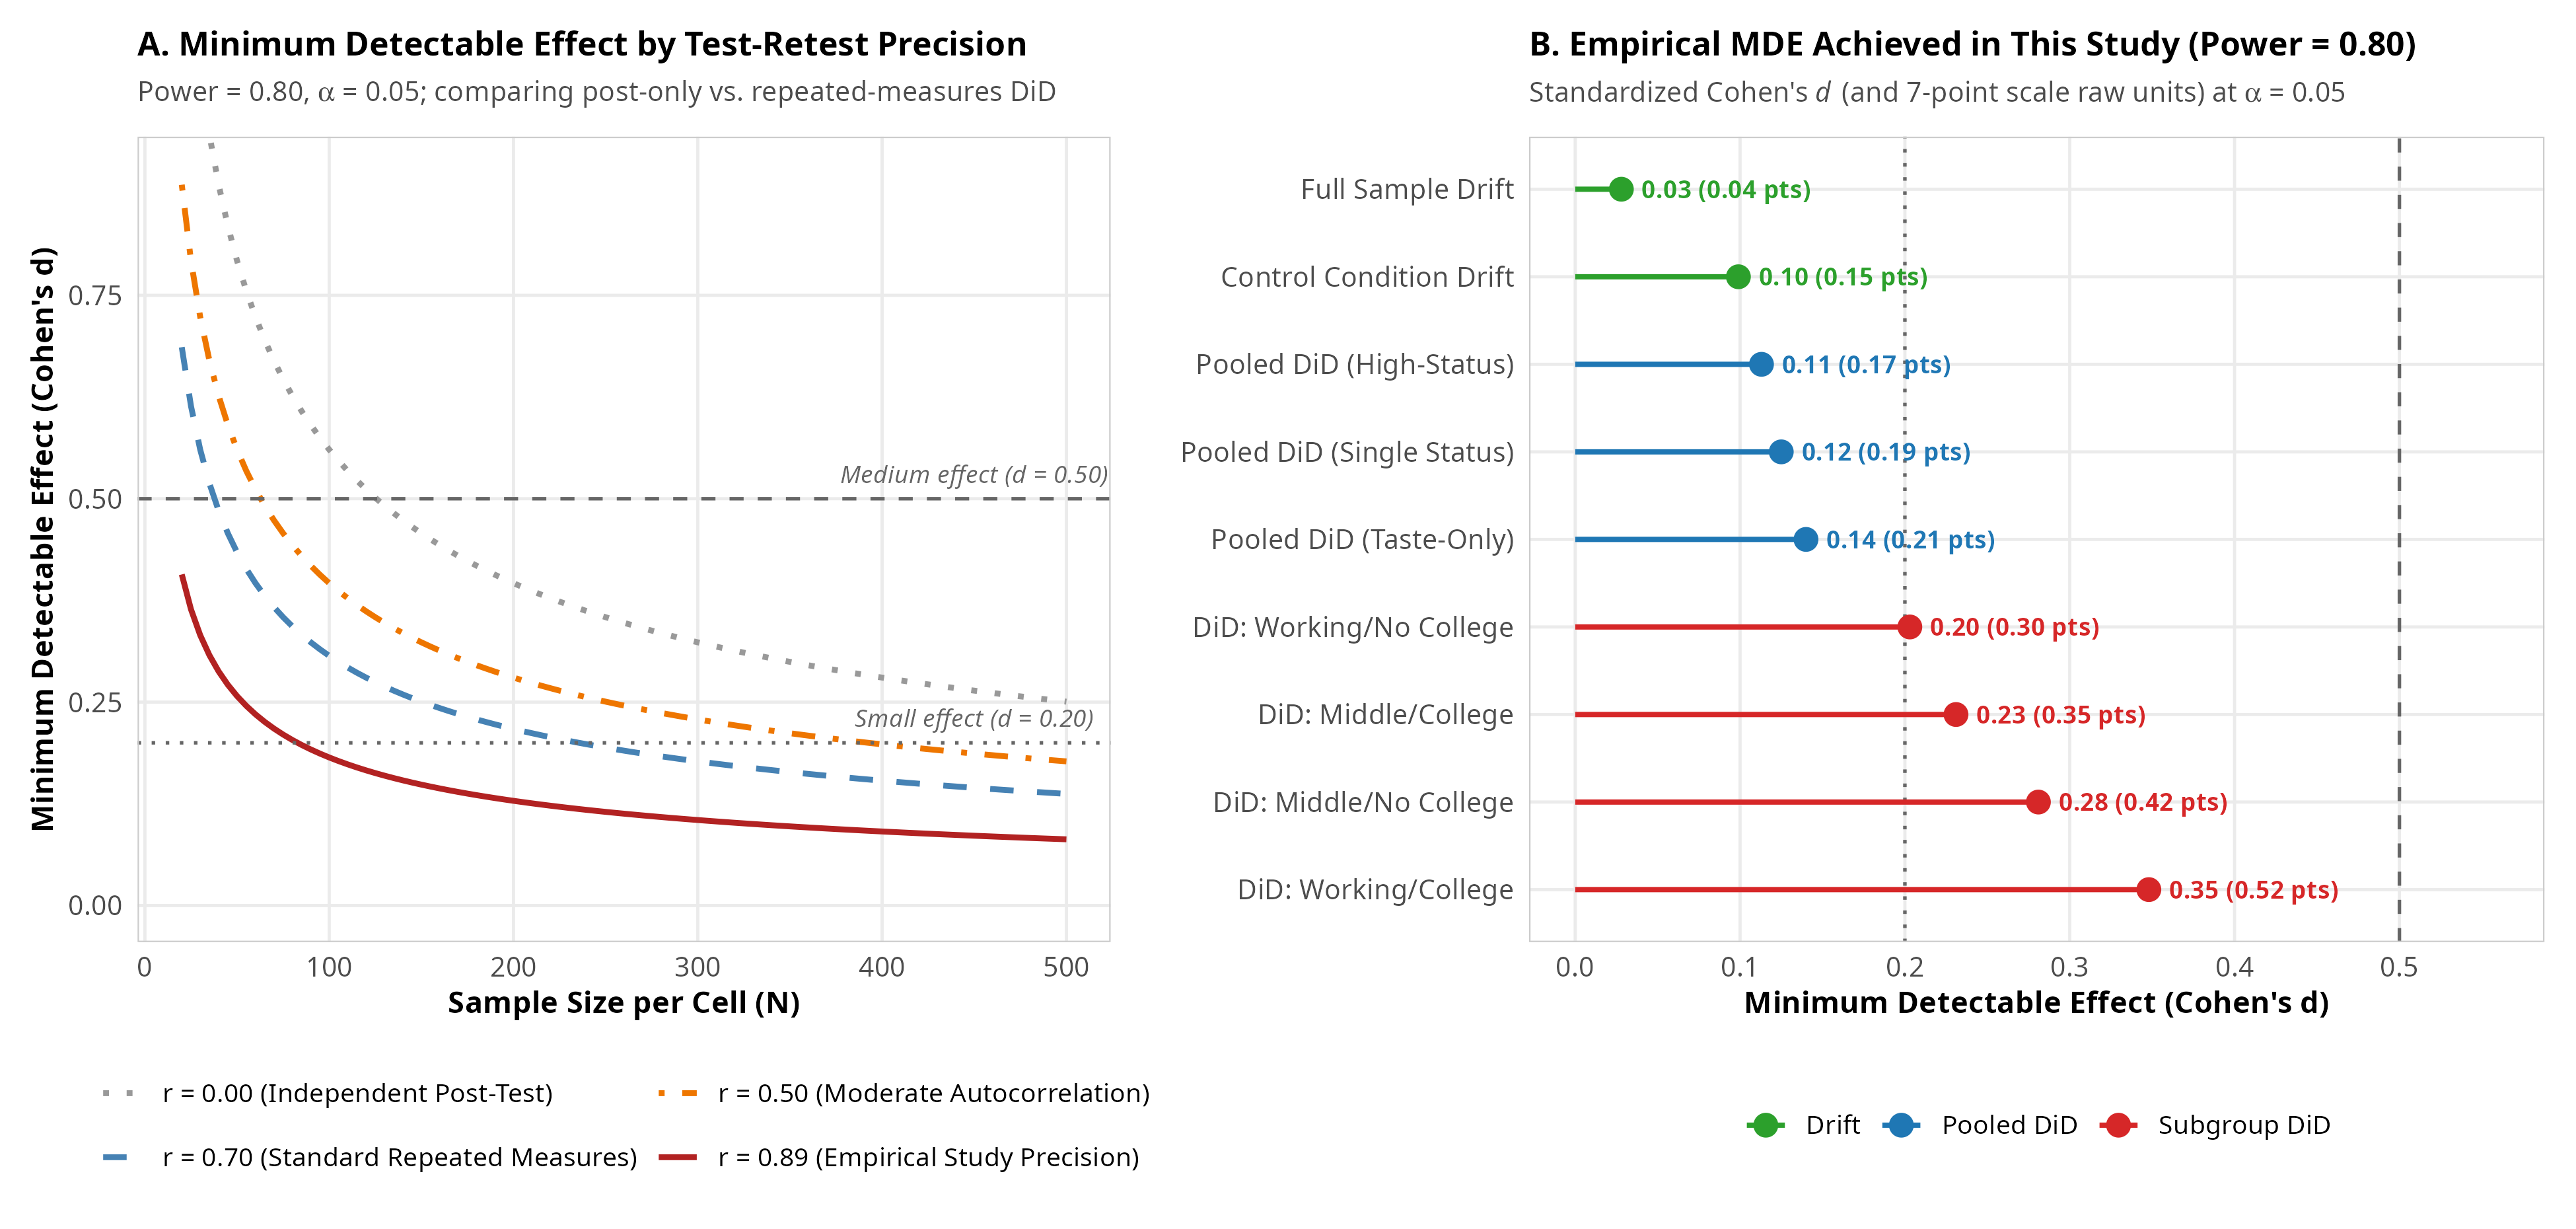
\includegraphics[width=0.98\textwidth]{figures/Figure_MDE_Power_Curves.png}
    \caption{Minimum Detectable Effect (MDE) Power Analysis. Panel A displays theoretical MDE curves (Cohen's $d$) at 80\% power ($\alpha = 0.05$) across cell sample sizes, illustrating the precision advantage of repeated-measures DiD across varying levels of test-retest autocorrelation ($r$). Panel B displays the empirical MDE thresholds achieved in this study across within-subject drift benchmarks, pooled DiD models, and status-differentiated subgroup comparisons.}
    \label{fig:mde_curves}
\end{figure}

The empirical findings from the MDE analysis yield three primary methodological takeaways. First, regarding repeated-measures exposure drift (Panel A of Table \ref{tbl:mde_analysis}), the full sample ($N = 2,253$) possessed extraordinary statistical power, capable of detecting shifts as minute as Cohen's $d \ge 0.028$ (0.041 scale points). Crucially, even within the unexposed Control Condition ($N_C = 177$), the design was powered at 80\% to detect drift as small as $d \ge 0.099$ (0.148 scale points). This high baseline precision enabled us to reliably identify the empirical $+0.107$ exposure drift in the Control Condition ($t = 2.05, p = 0.041$), confirming that the upward drift was not an artifact of random noise.

Second, for the primary pooled Difference-in-Differences models benchmarked against the unexposed Control Condition (Panel B of Table \ref{tbl:mde_analysis}), the design possessed 80\% power to detect small treatment effects: $d \ge 0.113$ (0.169 points) for pooled high-status conditions ($N_T = 575$), $d \ge 0.125$ (0.188 points) for single-status conditions ($N_T \approx 290$), and $d \ge 0.140$ (0.210 points) for taste-only conditions ($N_T = 172$). All three pooled thresholds fall comfortably below Cohen's standard threshold for a ``small'' effect size ($d = 0.20$). This confirms that the pooled models were well-equipped to detect subtle social influence cues.

Third, within the disaggregated status consistency quadrants (Panel C of Table \ref{tbl:mde_analysis}), cell sizes are necessarily smaller, leading to wider detection envelopes. In the two larger, status-consistent quadrants—Working Class without College ($N_C = 70$) and Middle Class with College ($N_C = 51$)—the median MDE thresholds were $d = 0.203$ (0.304 scale points) and $d = 0.231$ (0.347 scale points), providing adequate power for small-to-moderate effects. In contrast, in the smaller, status-inconsistent quadrants—Middle Class without College ($N_C = 33$) and Working Class with College ($N_C = 23$)—the median MDE thresholds expanded to $d = 0.281$ (0.421 points) and $d = 0.348$ (0.522 points). Consequently, statistically significant shifts in these cells emerged only when behavioral adjustments were pronounced, such as the $-0.394$ negative divergence ($p < 0.001$) observed among college-educated working-class respondents exposed to High-Status Dislike cues. Methodologically, this indicates that non-significant coefficients within the smallest status cells should be interpreted as reflecting wider estimation uncertainty rather than definitive evidence of null influence.

\section{Survey Vignettes and Treatment Prompts}
\label{sec:appendix_vignettes}
Below we transcribe the verbatim wording and sequencing of the survey instrument administered in the 2012 study, based on the original Qualtrics protocol.

\subsection*{1. Baseline Measurement (Trial 1)}
Respondents were presented with the high-resolution image of James McNeill Whistler's \textit{Nocturne: Blue and Gold -- Old Battersea Bridge} (1872) and asked:
\begin{quote}
\textit{``Please look at this painting for a few seconds. Give us your first impression of this painting -- how much do you like it?''}
\end{quote}
Responses were recorded on a 7-point Likert scale: 1 = ``I like it very much'', 2 = ``I like it'', 3 = ``I like it just a little'', 4 = ``I neither like it nor dislike it'', 5 = ``I dislike it just a little'', 6 = ``I dislike it'', and 7 = ``I dislike it very much'' (plus a visual filter option ``I can't see the image''). Items were reverse-coded in data processing so that 7 indicates highest affinity and 1 indicates lowest affinity.

\subsection*{2. Experimental Treatment Vignettes}
Following their initial evaluation, respondents assigned to experimental conditions were exposed to feedback from others. Notably, the prompt did \textit{not} describe the evaluating group in relative terms to the participant; instead, it presented absolute descriptive characteristics of the alter group, allowing social proximity or distance to emerge relationally from the participant's own social location.

In the Treatment Conditions combining class status and taste information, respondents read:
\begin{quote}
\textit{``Thank you for your response. Our survey so far indicates that the group of people most likely to say that they [LIKE / DISLIKE] the painting you saw have completed\dots''}
\end{quote}
For Low Cultural Capital (LCC) others, the description read: \textit{``\dots high school but did not go to college, and work in a food service job.''} For Economic Specialists (ES / High Cultural Capital), it read: \textit{``\dots a Bachelor's degree in Business but no additional degrees, and work at a financial investment firm.''} For Cultural Specialists (CS / High Cultural Capital), it read: \textit{``\dots several advanced degrees including a PhD, and work at a college or university.''}

Immediately following the vignette, respondents were asked: \textit{``Given only what you know about this group's education, occupation, and opinion about the painting, how similar do you think you are to the people in this group?''} (with response options: Very similar, Somewhat similar, Just a little similar, Not very similar, or Not at all similar). Treatment respondents then answered an attribution probe: \textit{``In the last question, when you thought about how similar you are to the people in this group, which factor was most influential?''} (with options: Their education and/or occupation, Their opinion about the painting, or A combination of both).

In the Taste-Only Control Condition, respondents were told: \textit{``Thank you for your response. Other people who have taken this survey recently have said that they [LIKE / DISLIKE] the painting you saw. Given only what you know about these people's opinion about the painting, how similar do you think you are to them?''} Finally, respondents in the pure No-Alter Control Condition received no feedback screen or cues from others whatsoever, proceeding directly to the intervening survey block.

\subsection*{3. Intervening Survey Battery}
Between Trial 1 and Trial 2, all respondents completed substantive survey sections comprising full educational history (highest degree attained and college major field), intergenerational educational capital (parental bachelor's degree attainment), employment status and detailed 22-category Standard Occupational Classification (SOC), annual personal pre-tax income (23 income brackets), subjective social class self-identification (Lower class, Working class, Middle class, Upper class), and an extensive musical taste battery assessing liking, listening frequency, favorite genre, and perceived audience stereotypes across 20 musical genres.

\subsection*{4. Post-Treatment Measurement (Trial 2)}
Following the intervening modules, respondents were re-shown the identical artwork and asked:
\begin{quote}
\textit{``Please look at this painting for a few seconds again. Give us your final impression of this painting -- how much do you like it?''}
\end{quote}
recorded on the identical 7-point Likert scale.

\section{Comparison of Unweighted and IPW-Weighted Pooled DiD Models}
\label{sec:appendix_ipw_compare}
Table \ref{tbl:appendix_did_compare} reports the side-by-side comparison between the primary unweighted DiD model and the IPW-weighted model balancing baseline age, gender, race/ethnicity, and parental education across the pooled sample. Both specifications produce consistent point estimates, standard errors, and substantive conclusions regarding valence asymmetry and exposure drift suppression.

\begin{table}[ht!]
\centering
\small
\caption{Comparison of Unweighted and IPW-Weighted Difference-in-Differences Models (Pooled Sample)}
\label{tbl:appendix_did_compare}
\setlength{\tabcolsep}{4.5pt}
\begin{tabular*}{\linewidth}{@{\extracolsep{\fill}}lcccc@{}}
\toprule
 & \multicolumn{2}{c}{\textbf{Unweighted DiD}} & \multicolumn{2}{c}{\textbf{IPW-Weighted DiD}} \\
\cmidrule(lr){2-3} \cmidrule(lr){4-5}
\textbf{Independent Variable} & Estimate (SE) & $t$ value & Estimate (SE) & $t$ value \\
\midrule
Intercept ($\beta_0$) & 4.689 (0.114) & 40.99$^{***}$ & 4.672 (0.115) & 40.72$^{***}$ \\
Trial 2 Exposure Drift ($\beta_{1}$) & 0.107 (0.052) & 2.05$^{*}$ & 0.156 (0.054) & 2.90$^{**}$ \\
\addlinespace[3pt]
\multicolumn{5}{l}{\textit{Difference-in-Differences Treatment Effects ($\text{Trial} \times \text{Condition}$):}} \\
\quad Class \& Taste / Dislike / $+$Status & $-0.121$ (0.060) & $-2.02^{*}$ & $-0.201$ (0.062) & $-3.27^{**}$ \\
\quad Class \& Taste / Like / $-$Status & $-0.128$ (0.067) & $-1.93^{\dagger}$ & $-0.112$ (0.069) & $-1.61$ \\
\quad Taste Only / Dislike & $-0.125$ (0.075) & $-1.67^{\dagger}$ & $-0.172$ (0.076) & $-2.26^{*}$ \\
\quad Class \& Taste / Like / $+$Status & $+0.041$ (0.060) & 0.68 & $+0.006$ (0.062) & 0.09 \\
\quad Taste Only / Like & $+0.096$ (0.075) & 1.29 & $+0.068$ (0.078) & 0.87 \\
\quad Class \& Taste / Dislike / $-$Status & $+0.016$ (0.066) & 0.23 & $-0.034$ (0.068) & $-0.49$ \\
\addlinespace[3pt]
Condition Main Effects Included & \multicolumn{2}{c}{Yes} & \multicolumn{2}{c}{Yes} \\
Random Intercept Variance ($\sigma^2_u$) & \multicolumn{2}{c}{2.074} & \multicolumn{2}{c}{2.026} \\
Residual Variance ($\sigma^2_e$) & \multicolumn{2}{c}{0.243} & \multicolumn{2}{c}{1.022} \\
$N$ (Observations / Individuals) & \multicolumn{2}{c}{4,506 / 2,253} & \multicolumn{2}{c}{4,504 / 2,252} \\
\bottomrule
\end{tabular*}
\begin{minipage}{\linewidth}
\vspace{4pt}
\footnotesize
\textit{Note:} $^{\dagger}p < 0.10, ^{*}p < 0.05, ^{**}p < 0.01, ^{***}p < 0.001$. Reference condition: unexposed Control Condition.
\end{minipage}
\end{table}

\begin{figure}[ht!]
    \centering
    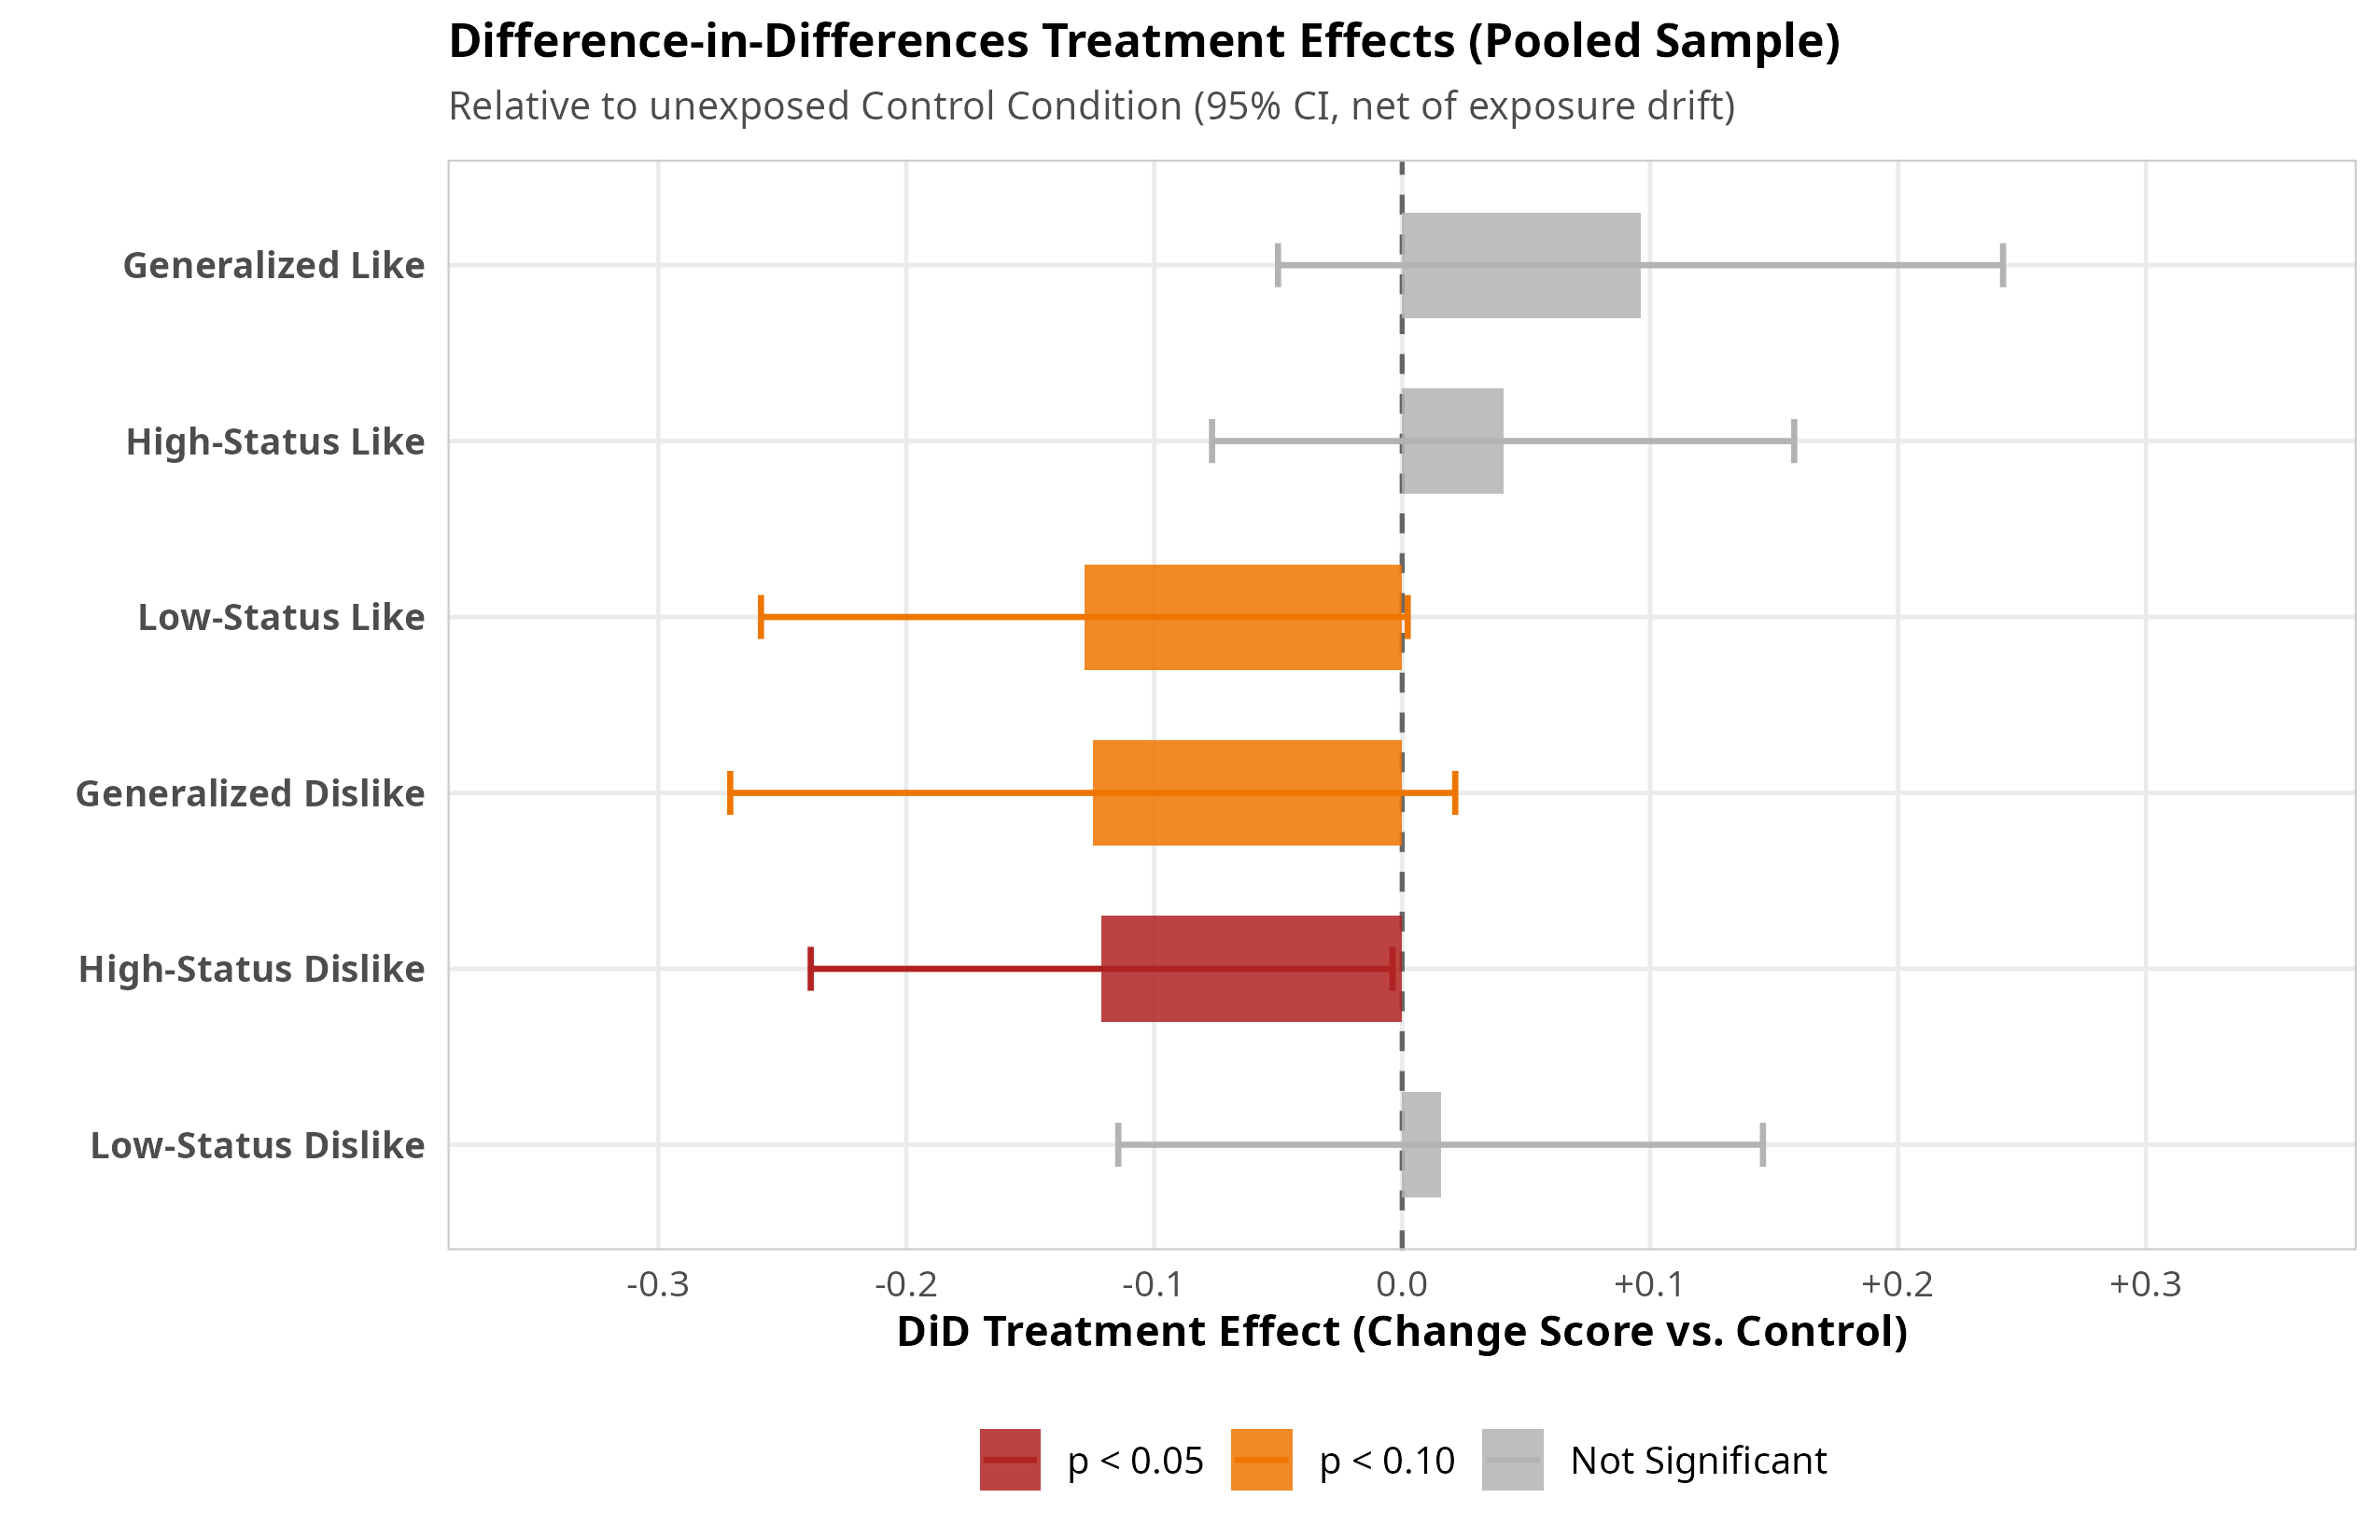
\includegraphics[width=0.88\textwidth]{figures/Figure_DiD_Pooled.png}
    \caption{Difference-in-Differences Treatment Effects in the Pooled Sample (Unweighted Linear Mixed Model). Horizontal bars denote point estimates with 95\% confidence intervals relative to the unexposed Control Condition (dashed line at zero). Colors indicate statistical significance: red ($p < 0.05$), orange ($p < 0.10$), and grey ($p \ge 0.10$).}
    \label{fig:did_pooled}
\end{figure}

\section{Complete Status-Differentiated DiD Estimates Across All Cells}
\label{sec:appendix_full_grid}
Figure \ref{fig:did_status_full} displays the complete 24-cell grid of Difference-in-Differences treatment effect estimates across all six treatment conditions and all four status consistency quadrants, estimated using Inverse Probability Weighting (IPW). Bars indicate point estimates and error bars denote 95\% confidence intervals relative to the unexposed Control Condition within each status group.

\begin{figure}[ht!]
    \centering
    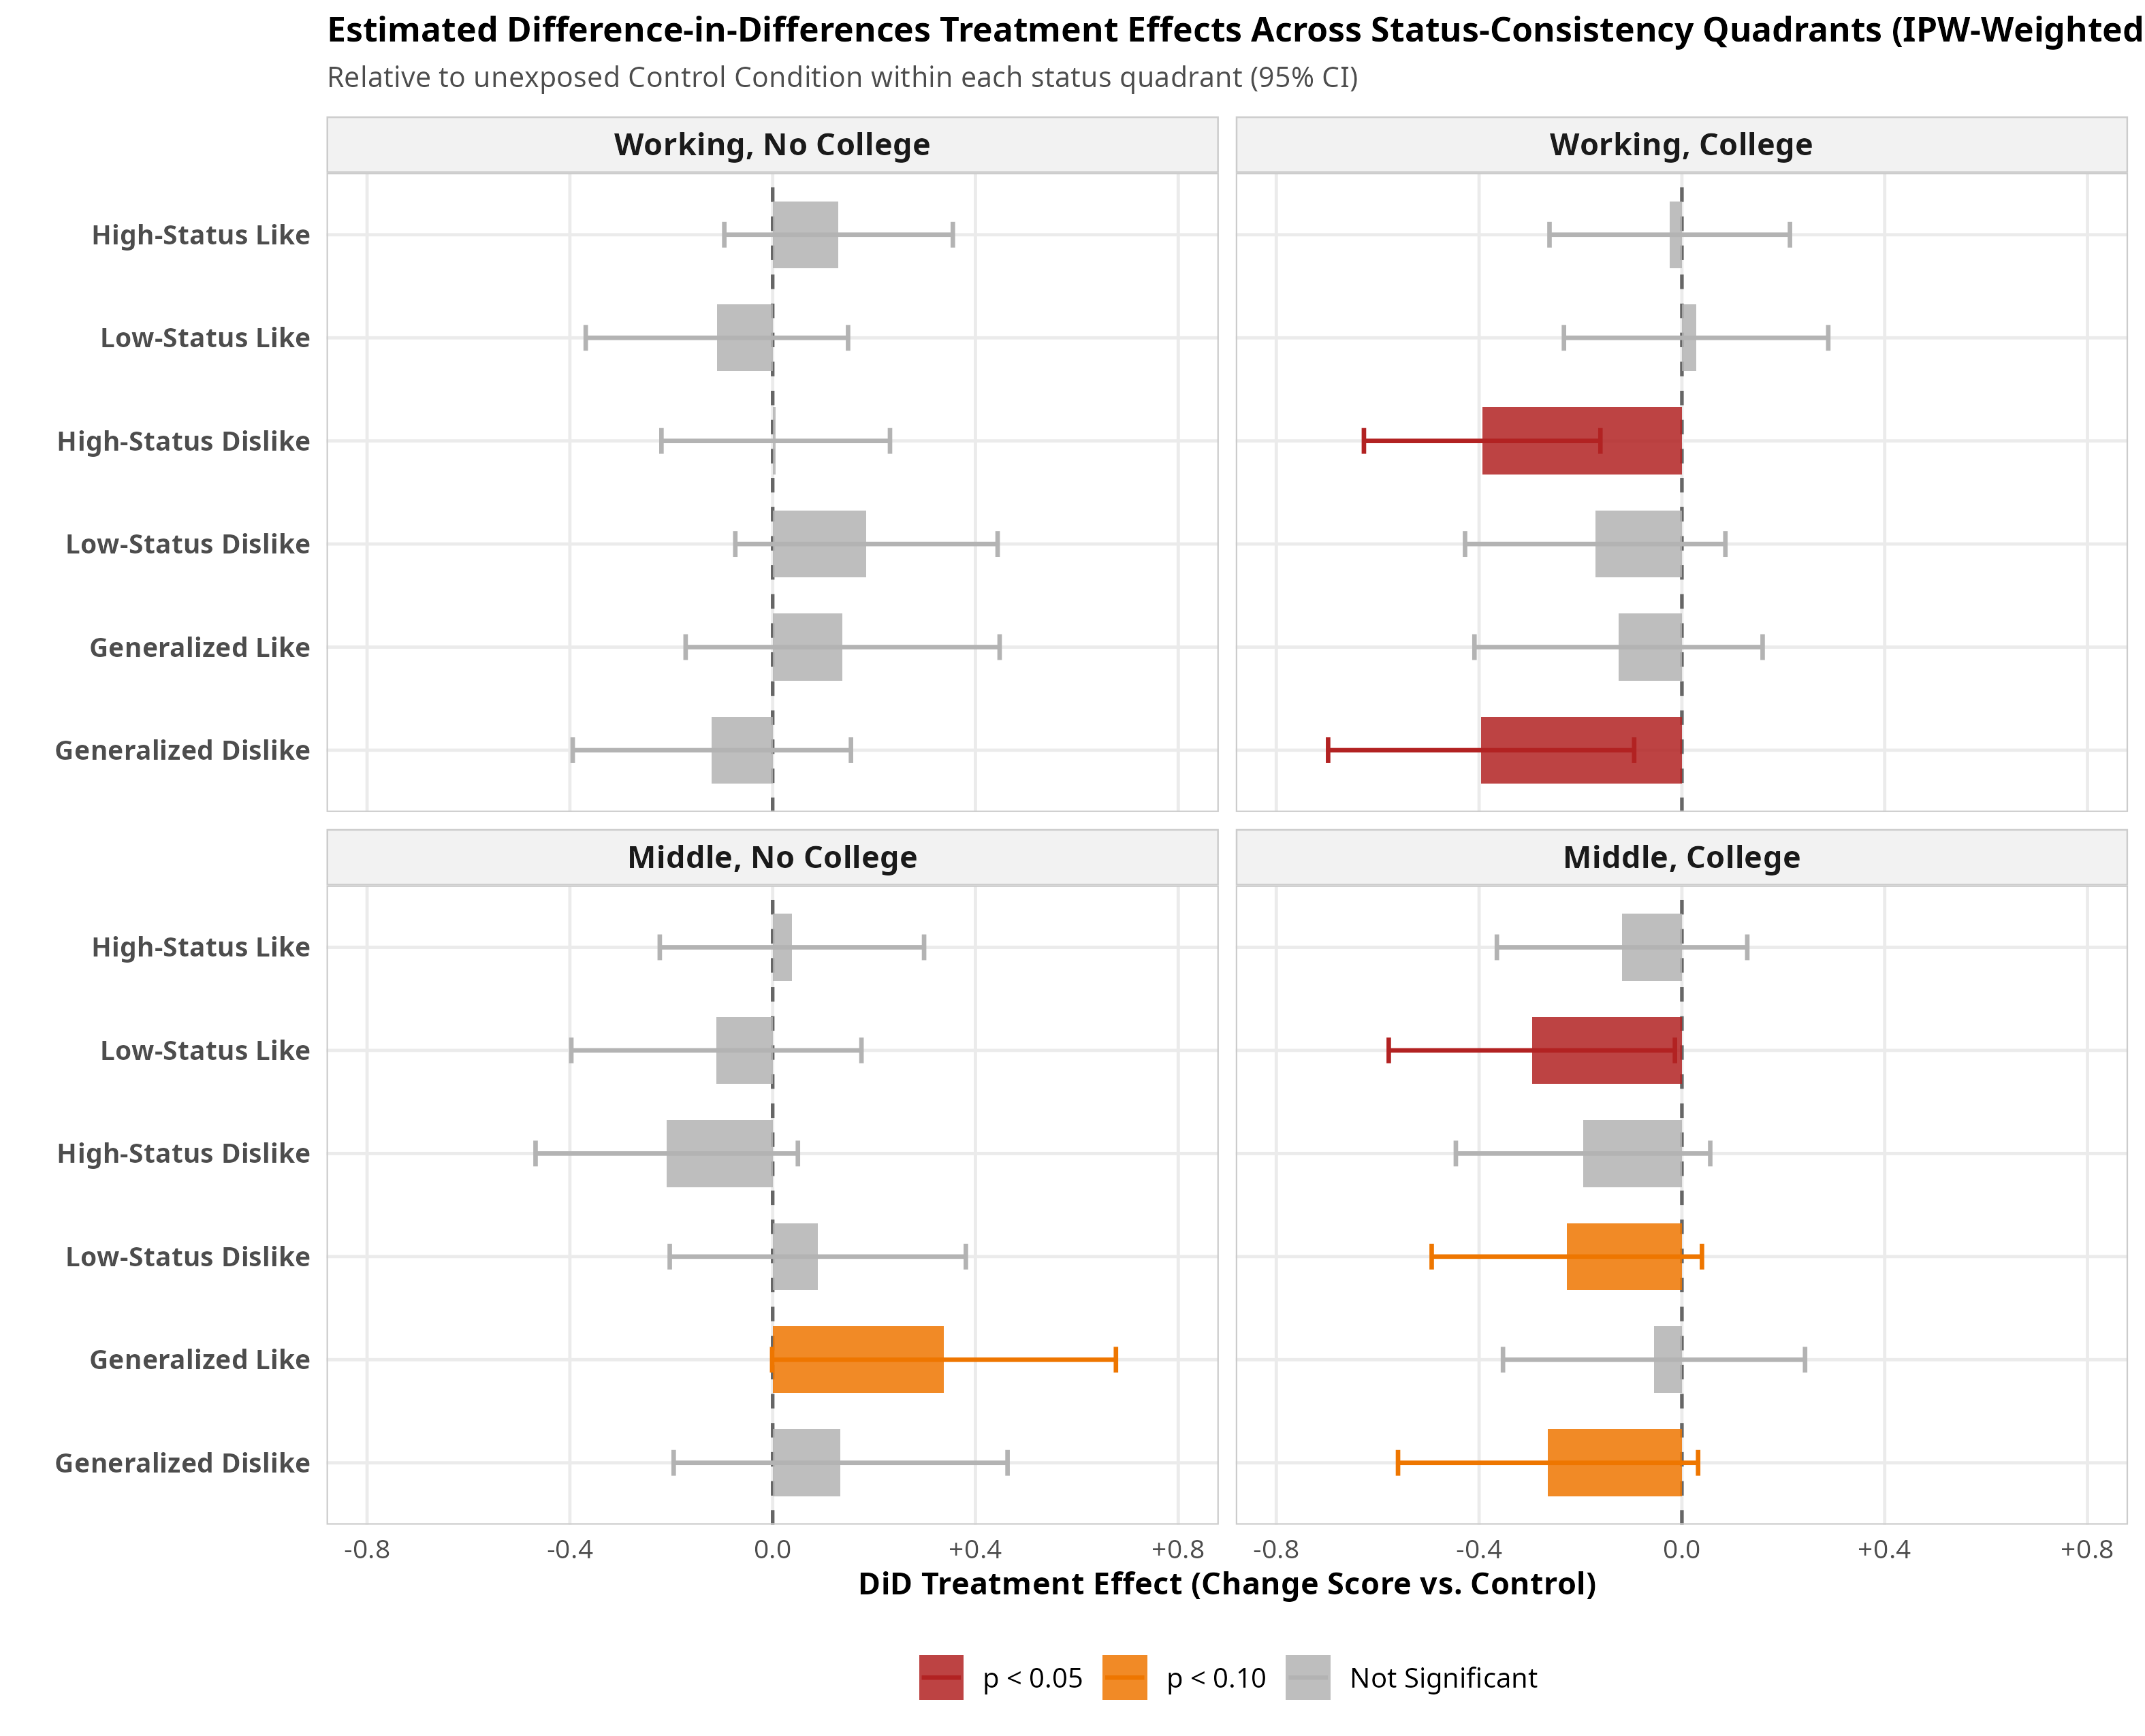
\includegraphics[width=0.95\textwidth]{figures/Figure_DiD_Status_All.png}
    \caption{Complete Grid of Difference-in-Differences Treatment Effects by Status Consistency Group (IPW-Weighted). Estimates benchmark condition shifts against the unexposed Control Condition. Colors indicate statistical significance: red ($p < 0.05$), orange ($p < 0.10$), and grey ($p \ge 0.10$).}
    \label{fig:did_status_full}
\end{figure}

\section{Sensitivity Analysis: Behavioral Choices Excluding Taste-Only Conditions}
\label{sec:appendix_sens_multinom}
To verify that the discrete behavioral patterns documented in the main text (Figure \ref{fig:multinom}) are specifically generated by status-differentiated social influence rather than undifferentiated taste consensus cues, we conducted a sensitivity analysis excluding respondents assigned to the two Taste-Only conditions ($N = 344$). The resulting analytic sample ($N = 1,870$) restricts behavioral classification strictly to respondents exposed to feedback combining evaluation valence and alter occupational/educational status, alongside unexposed control stayers.

Figure \ref{fig:sens_multinom} displays the Average Marginal Effects from this sensitivity specification, benchmarked against Working Class respondents without a college degree. As shown in the figure, all substantive patterns persist with exceptional stability: status-consistent college-educated respondents exhibit elevated evaluative stability ($\text{AME} = +0.048, p < 0.001$), status-inconsistent respondents exhibit heightened conformity ($\text{AME} = +0.060, p < 0.001$ for Working Class with College; $\text{AME} = +0.043, p < 0.001$ for Middle Class without College), and college education sharply reduces oppositional reactance ($\text{AME} = -0.030, p = 0.003$ and $\text{AME} = -0.021, p = 0.042$). Notably, under this status-restricted specification, the lower evaluative stability of status-inconsistent workers reaches full statistical significance ($\text{AME} = -0.030, p = 0.038$), reinforcing our core finding that status crystallization anchors aesthetic judgments against external social influence.

\begin{figure}[ht!]
    \centering
    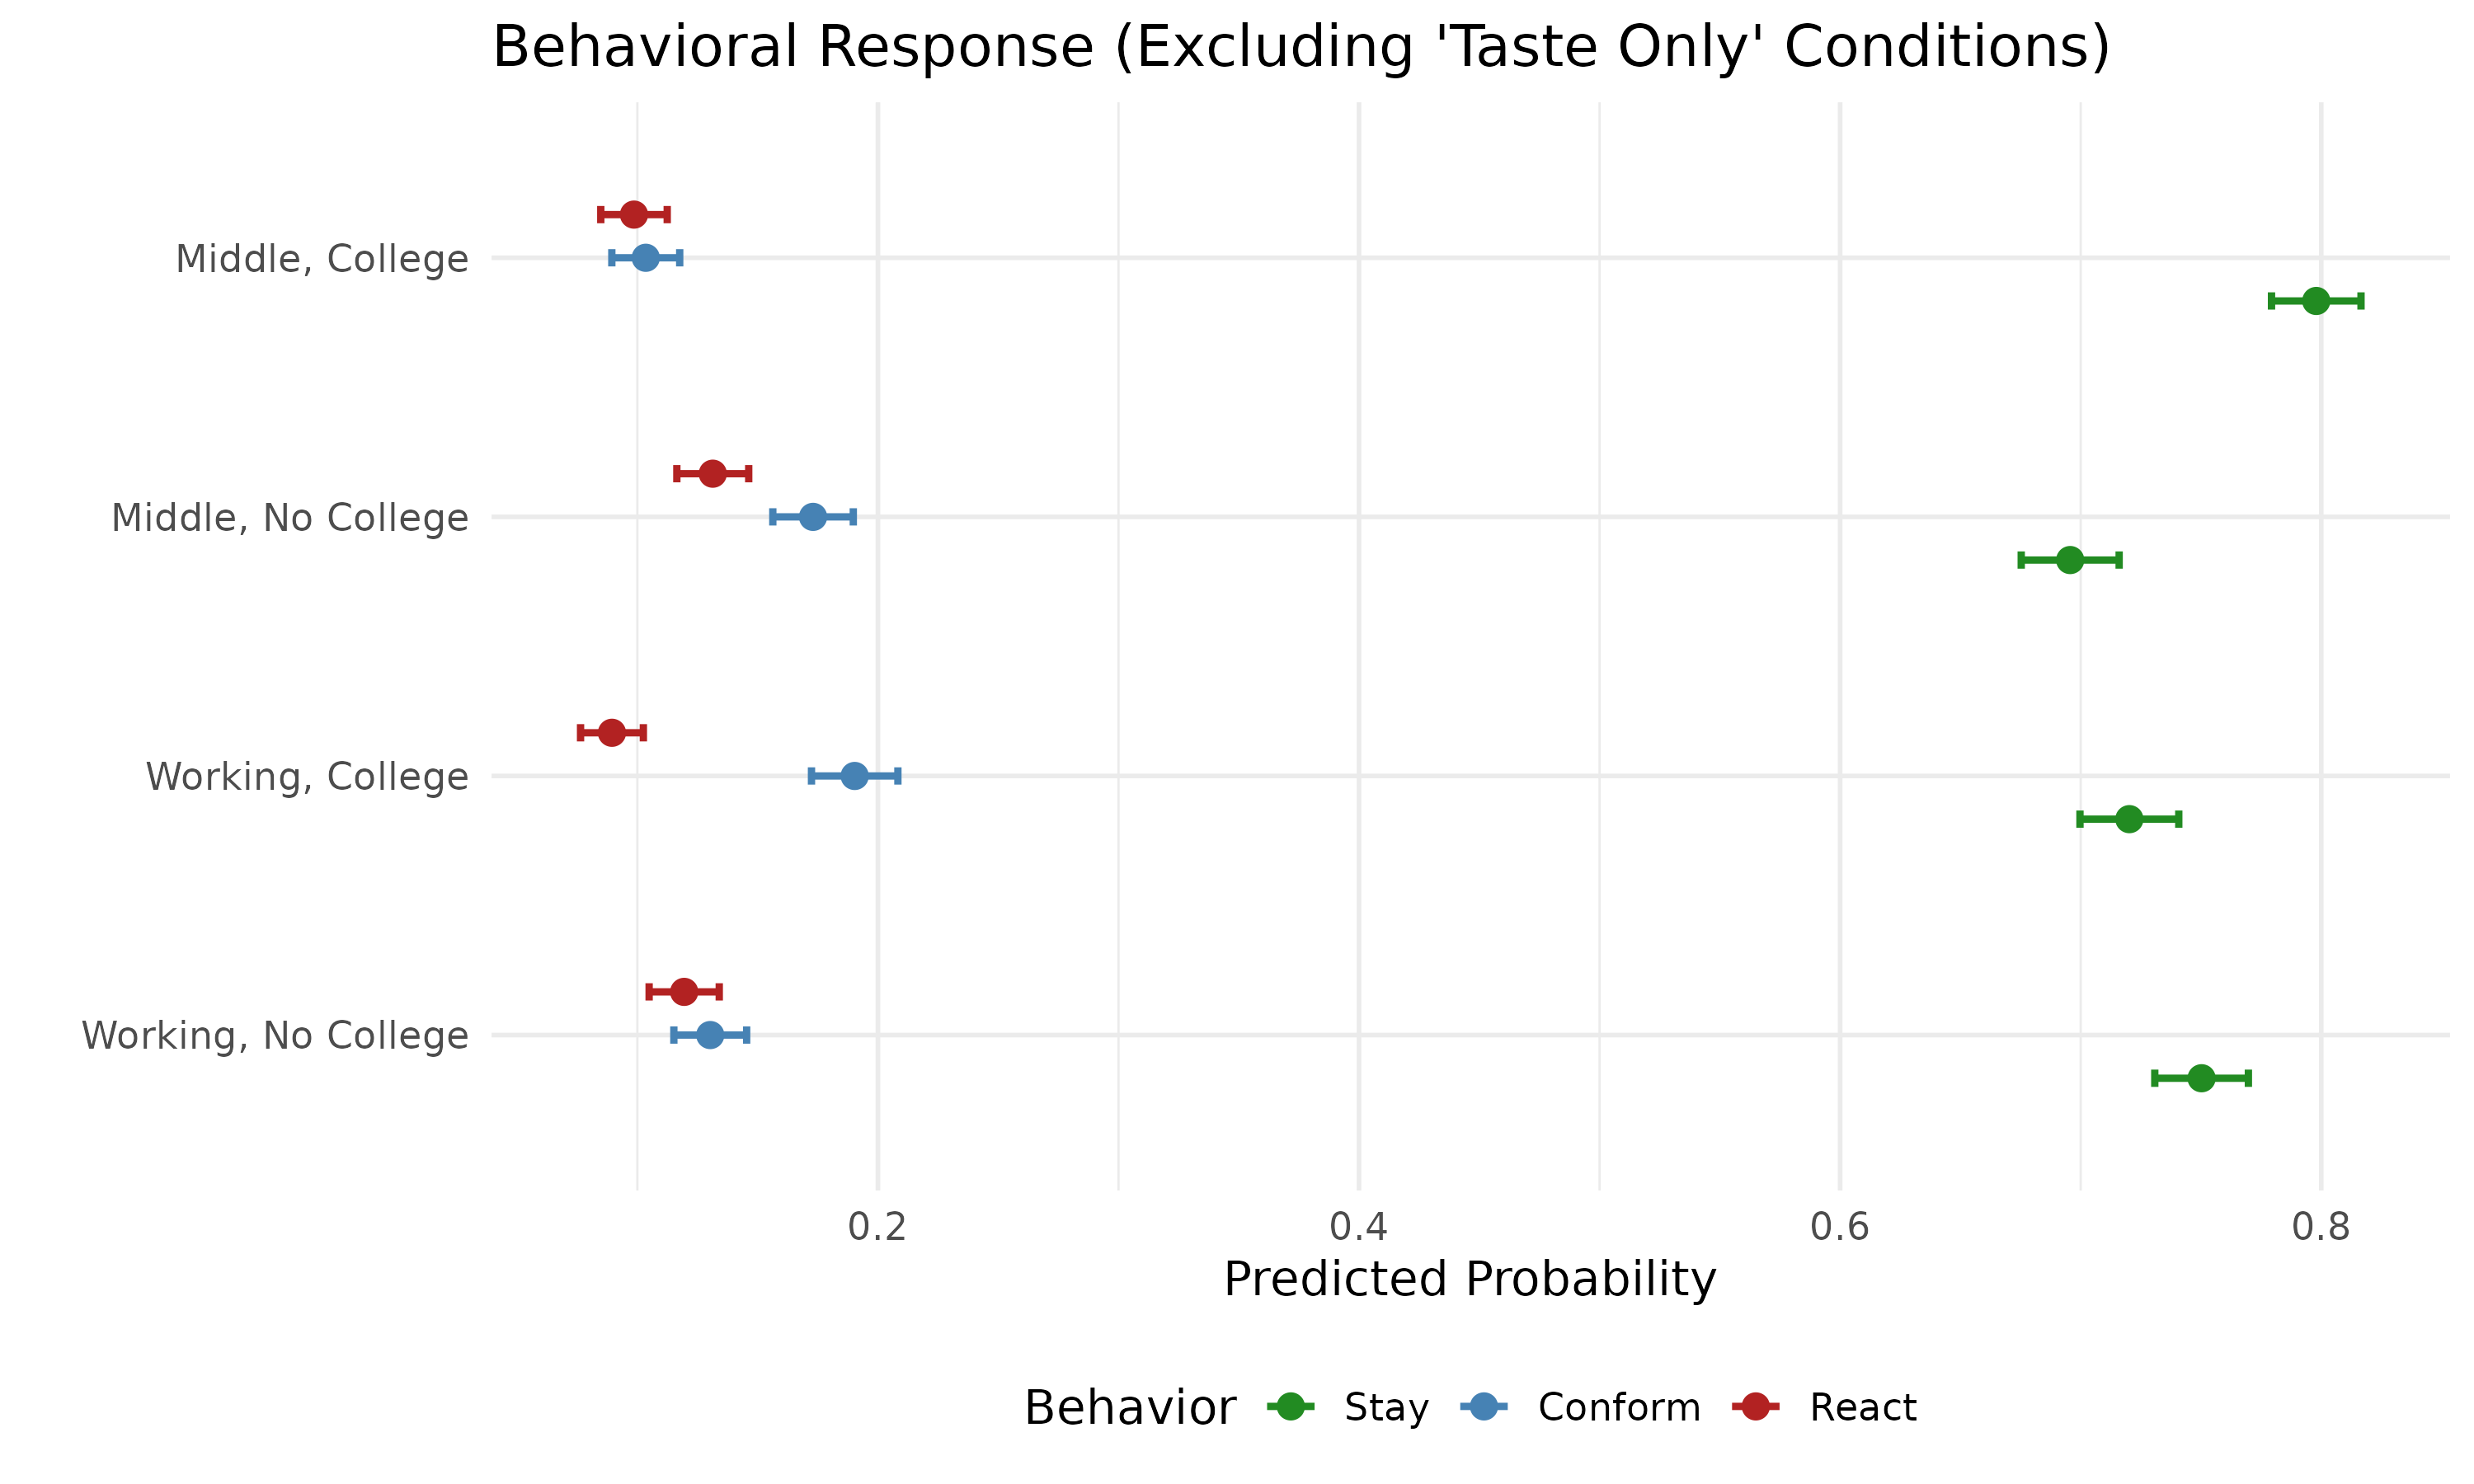
\includegraphics[width=0.95\textwidth]{figures/Figure11_Sens_MultinomialBehavior.png}
    \caption{Sensitivity Analysis: Average Marginal Effects on Behavioral Choices (Stay, Conform, React) Across Status Consistency Groups Excluding Taste-Only Conditions ($N = 1,870$). Horizontal bars indicate differences in choice probability relative to Working Class respondents without a college degree, with 95\% confidence intervals. Colors indicate statistical significance: red ($p < 0.05$) and grey ($p \ge 0.10$).}
    \label{fig:sens_multinom}
\end{figure}

\section{Robustness Check: Alternative Definition of Social Class}
\label{sec:appendix_class_robustness}
Restricting the subjective class definition strictly to respondents self-identifying as ``working class'' or ``middle class'' (excluding lower and upper class extremes) produces identical conclusions: status-consistent groups maintain the highest stay rates (Middle/College: 78.2\%; Working/No College: 74.7\%) and status-inconsistent groups maintain the highest conformity rates (Middle/No College: 17.9\%; Working/College: 16.9\%).

\end{document}
